%%%%%%%%%%%%%%%%%%%%%%%%%%%%%%%%%%%%%%%%%%%%%%%%%%%%%%%%%%%%%%
% Installation and demonstration
%%%%%%%%%%%%%%%%%%%%%%%%%%%%%%%%%%%%%%%%%%%%%%%%%%%%%%%%%%%%%%
\documentclass[../paper.tex]{subfiles}
\begin{document}
    To install the package from GitHub\footnote{\url{https://github.com/lechekhabm/GraphLab.jl}} and integrate it into the working environment, the following steps are required:

    \begin{enumerate}
        \item Add \texttt{GraphLab.jl} to the project using the Julia command:
\begin{lstlisting}[language = Julia]
using Pkg
Pkg.add(url="https://github.com/lechekhabm/GraphLab.jl")
\end{lstlisting}
        \item As a basic example for graph partitioning, the adjacency matrix $\mathbf{A}$ and vertex coordinates
        are first constructed from the input data.
        Here, we generate a synthetic $10 \times 50$ rectangular grid graph rotated by an angle of $\pi/3$ radians.
        Spectral bisection is then applied to compute the partition $p$, followed by visualization and export of the partitioned graph as an image. The process is executed with the following commands:
\begin{lstlisting}[language = Julia]
using GraphLab
A, coords = GraphLab.grid_graph(10, 50, π/3)
p = GraphLab.part_spectral(A)
GraphLab.draw_graph(A, coords, p, file_name="test.png")
\end{lstlisting}

        % The package automatically installs the following dependencies: \texttt{Arpack}, \texttt{CairoMakie}, \texttt{Colors}, \texttt{Graphs}, \texttt{LinearAlgebra}, \texttt{Metis}, \texttt{SparseArrays}, \texttt{Statistics}, \texttt{AMD}, \texttt{GraphsMatching}, \texttt{JuMP}, and \texttt{Cbc}.
        % For extended functionality, additional packages such as \texttt{DelimitedFiles}, \texttt{MAT}, \texttt{Plots}, and \texttt{PrettyTables} may be required.
    \end{enumerate}
Further details on the package and its functionalities can be found in the online documentation\footnote{\url{https://lechekhabm.github.io/GraphLab.jl/dev/}}.
    
%%%%%%%%%%%%%%%%%%%%%%%%%%%%%%%%%%%%%%%%%%%%%%%%%%%%%%%%%%%%%%
% Demonstration
%%%%%%%%%%%%%%%%%%%%%%%%%%%%%%%%%%%%%%%%%%%%%%%%%%%%%%%%%%%%%%
    % \subsection{Demonstration}
    % The package includes two example scripts that illustrate the usage of the framework for benchmarking and comparing various graph partitioning methods. These scripts are available in the `examples/` directory within the package and can be executed directly.



%%%%%%%%%%%%%%%%%%%%%%%%%%%%%%%%%%%%%%%%%%%%%%%%%%%%%%%%%%%%%%
% PLOT TEST
%%%%%%%%%%%%%%%%%%%%%%%%%%%%%%%%%%%%%%%%%%%%%%%%%%%%%%%%%%%%%%
% \begin{figure*}[!h]
% 	\centering
%     \subcaptionbox{\label{fig:LFR_Ncut}}
%     {\inputtikz{figures_tikz}{LFR_Fscore}}
% 	\caption{\label{fig:SBM_compare} Clustering the LFR datasets for an increasing noise component $\xi$. (a) NCut values. (b) Modularity values. (c) NMI accuracy values.}
% \end{figure*}


%%%%%%%%%%%%%%%%%%%%%%%%%%%%%%%%%%%%%%%%%%%%%%%%%%%%%%%%%%%%%%
% Ex 1
%%%%%%%%%%%%%%%%%%%%%%%%%%%%%%%%%%%%%%%%%%%%%%%%%%%%%%%%%%%%%%
    % \subsubsection{Example 1: Comparing partitioning methods}
    % This example compares various graph partitioning methods, including coordinate bisection, inertial bisection, spectral bisection and bisection using \texttt{METIS}. The script \texttt{ex1.jl} evaluates these methods across a series of different graphs, providing insights into their performance and effectiveness, as illustrated in \Cref{fig:ex1_results}. 
    % \begin{figure}[h]
    \centering
    \begin{subfigure}[b]{0.23\textwidth}
        \centering
        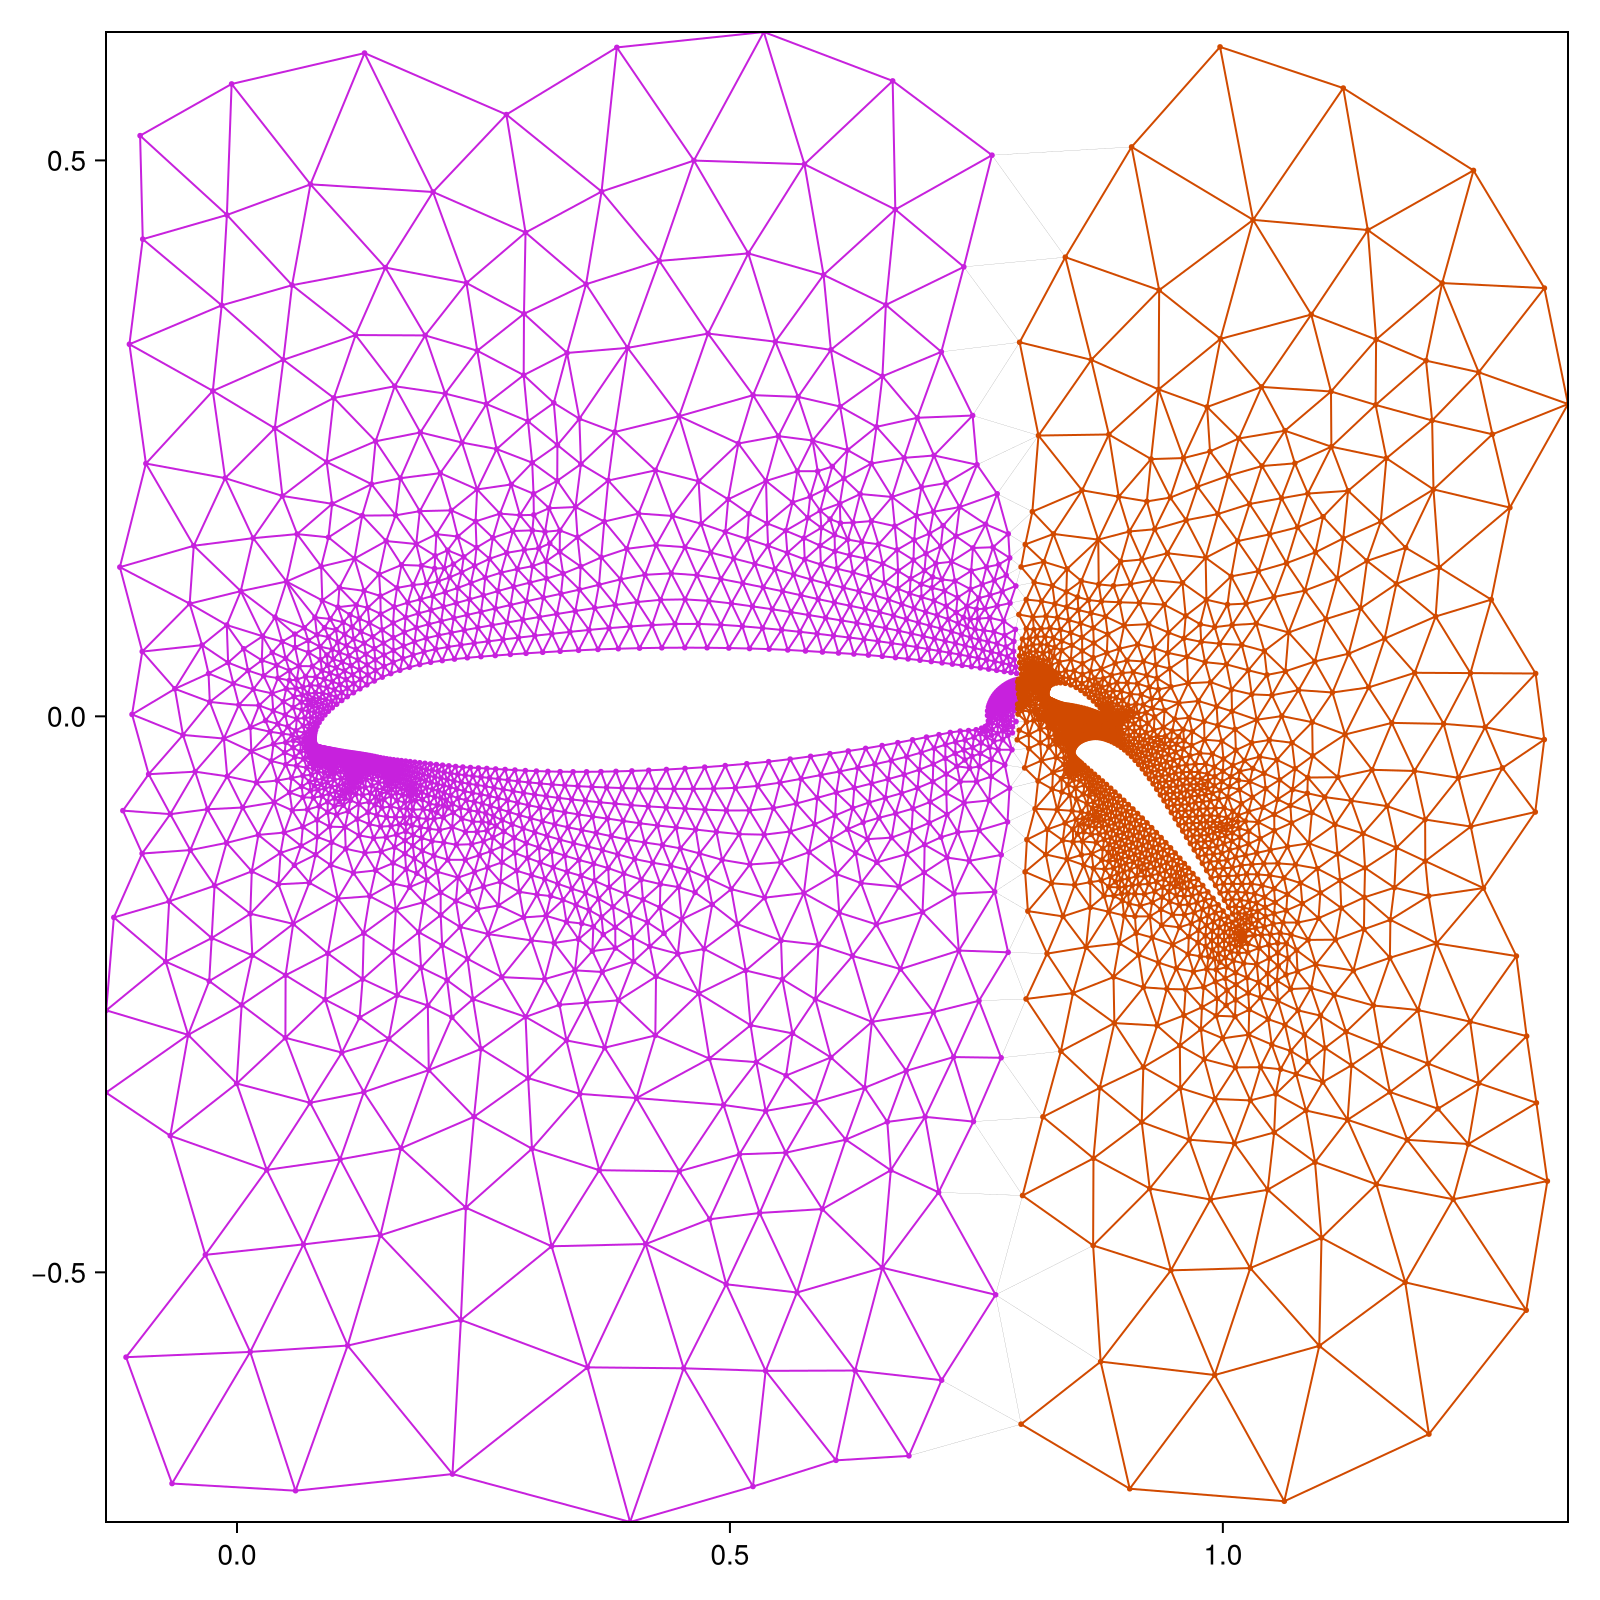
\includegraphics[width=\textwidth,  trim={100pt 74pt 0 0}, clip]{images/ex1_airfoil1_coordinate.png}
        \caption{Coordinate bisection}
        \label{fig:ex1_coord}
    \end{subfigure}
    \hfill
    \begin{subfigure}[b]{0.23\textwidth}
        \centering
        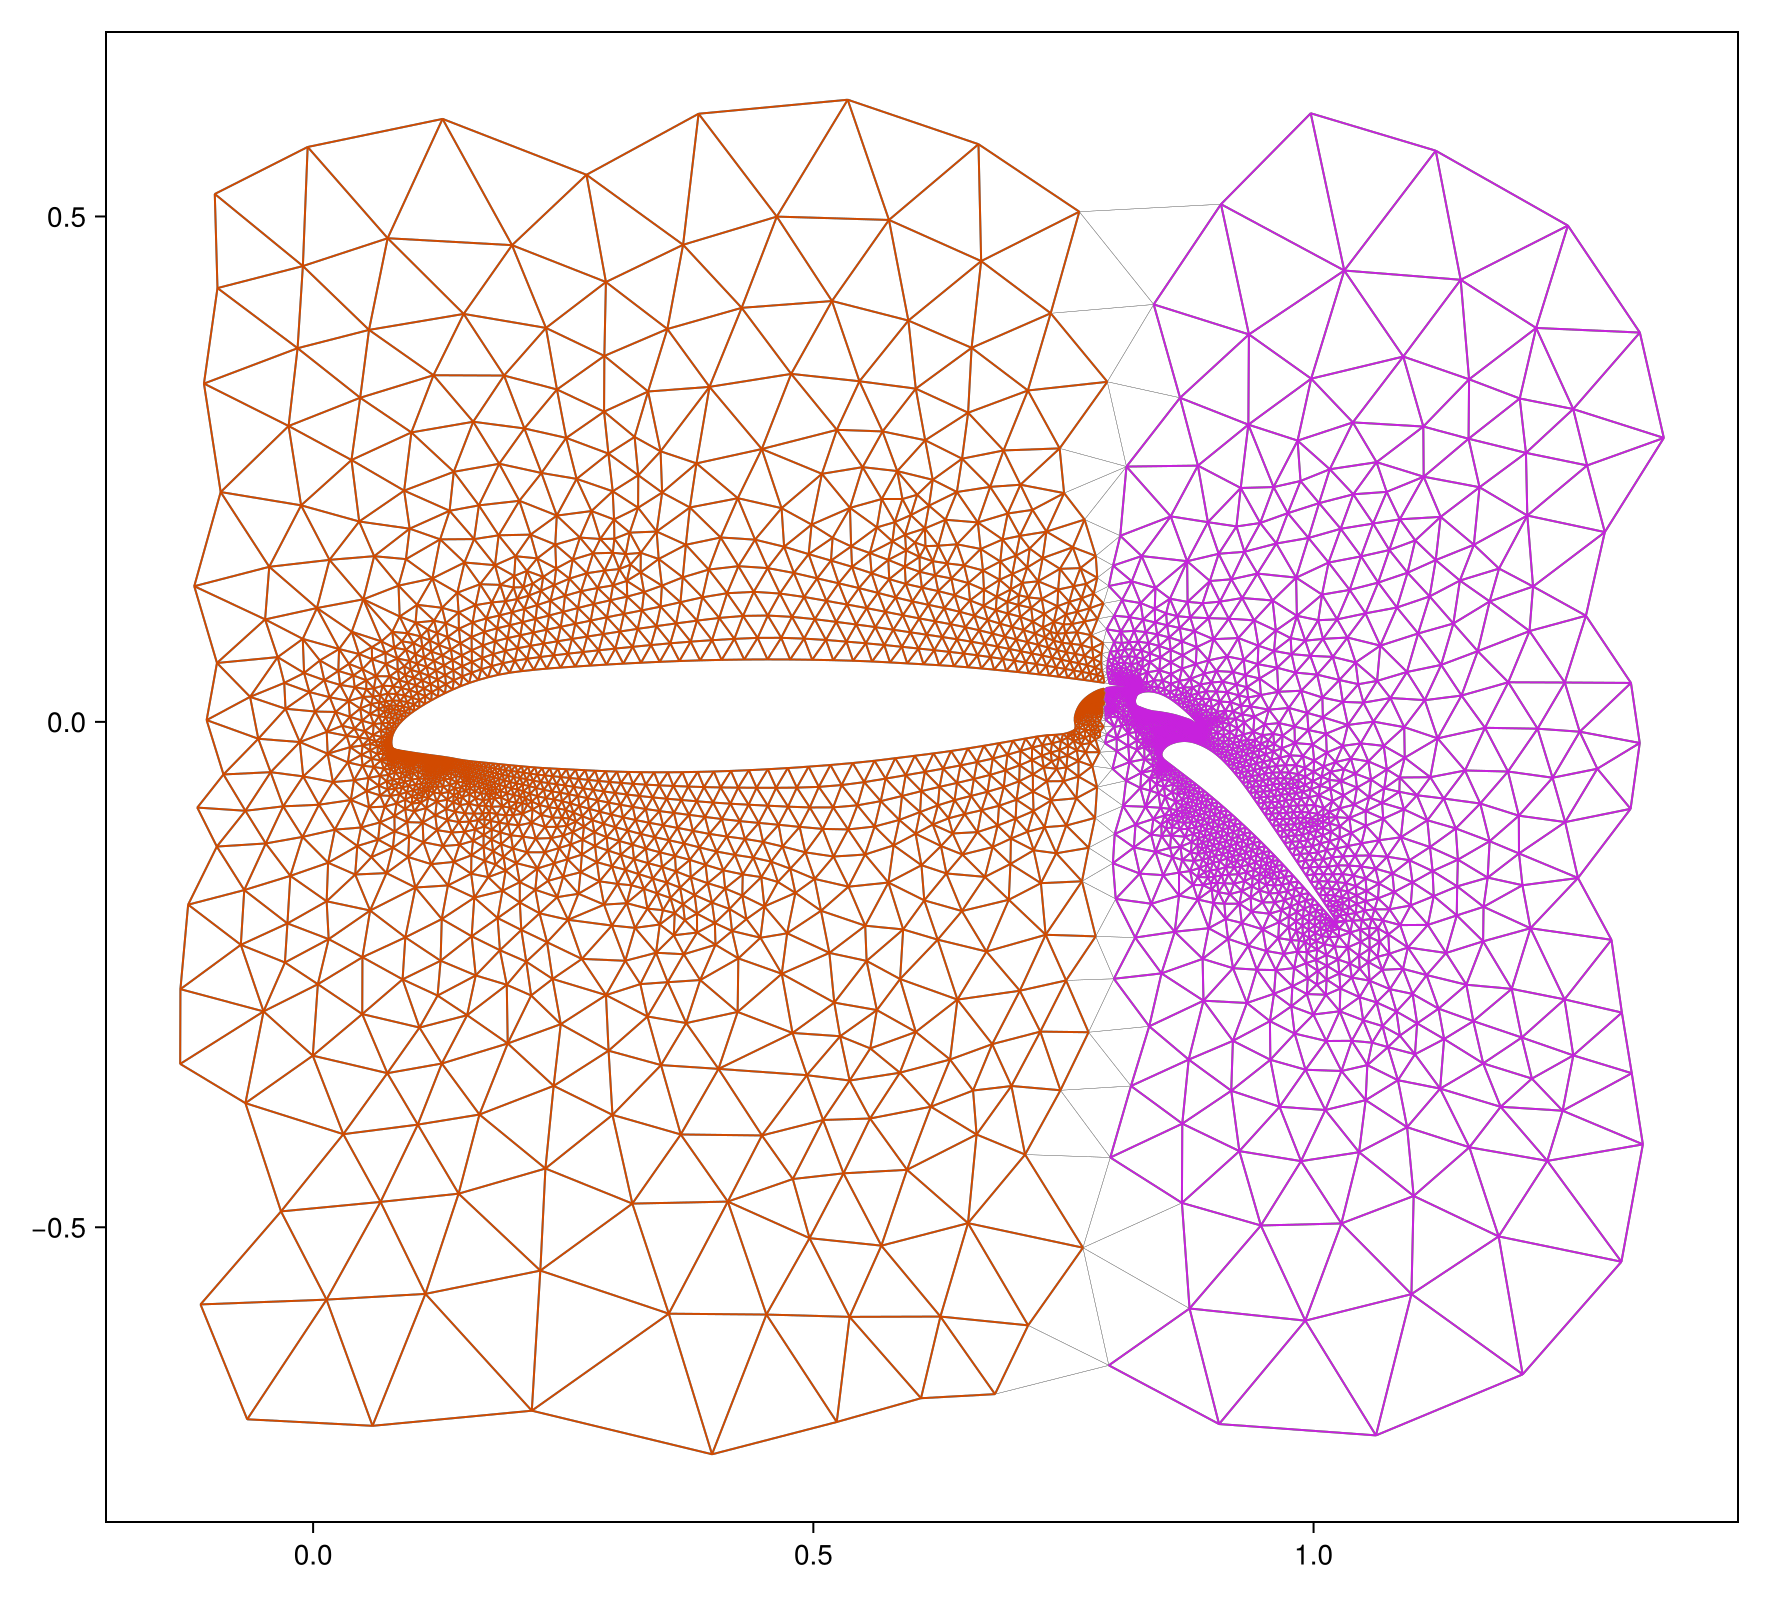
\includegraphics[width=\textwidth,  trim={100pt 74pt 0 0}, clip]{images/ex1_airfoil1_inertial.png}
        \caption{Inertial bisection}
        \label{fig:ex1_inertial}
    \end{subfigure}

    \vskip\baselineskip  % Adds vertical space between the rows

    \begin{subfigure}[b]{0.23\textwidth}
        \centering
        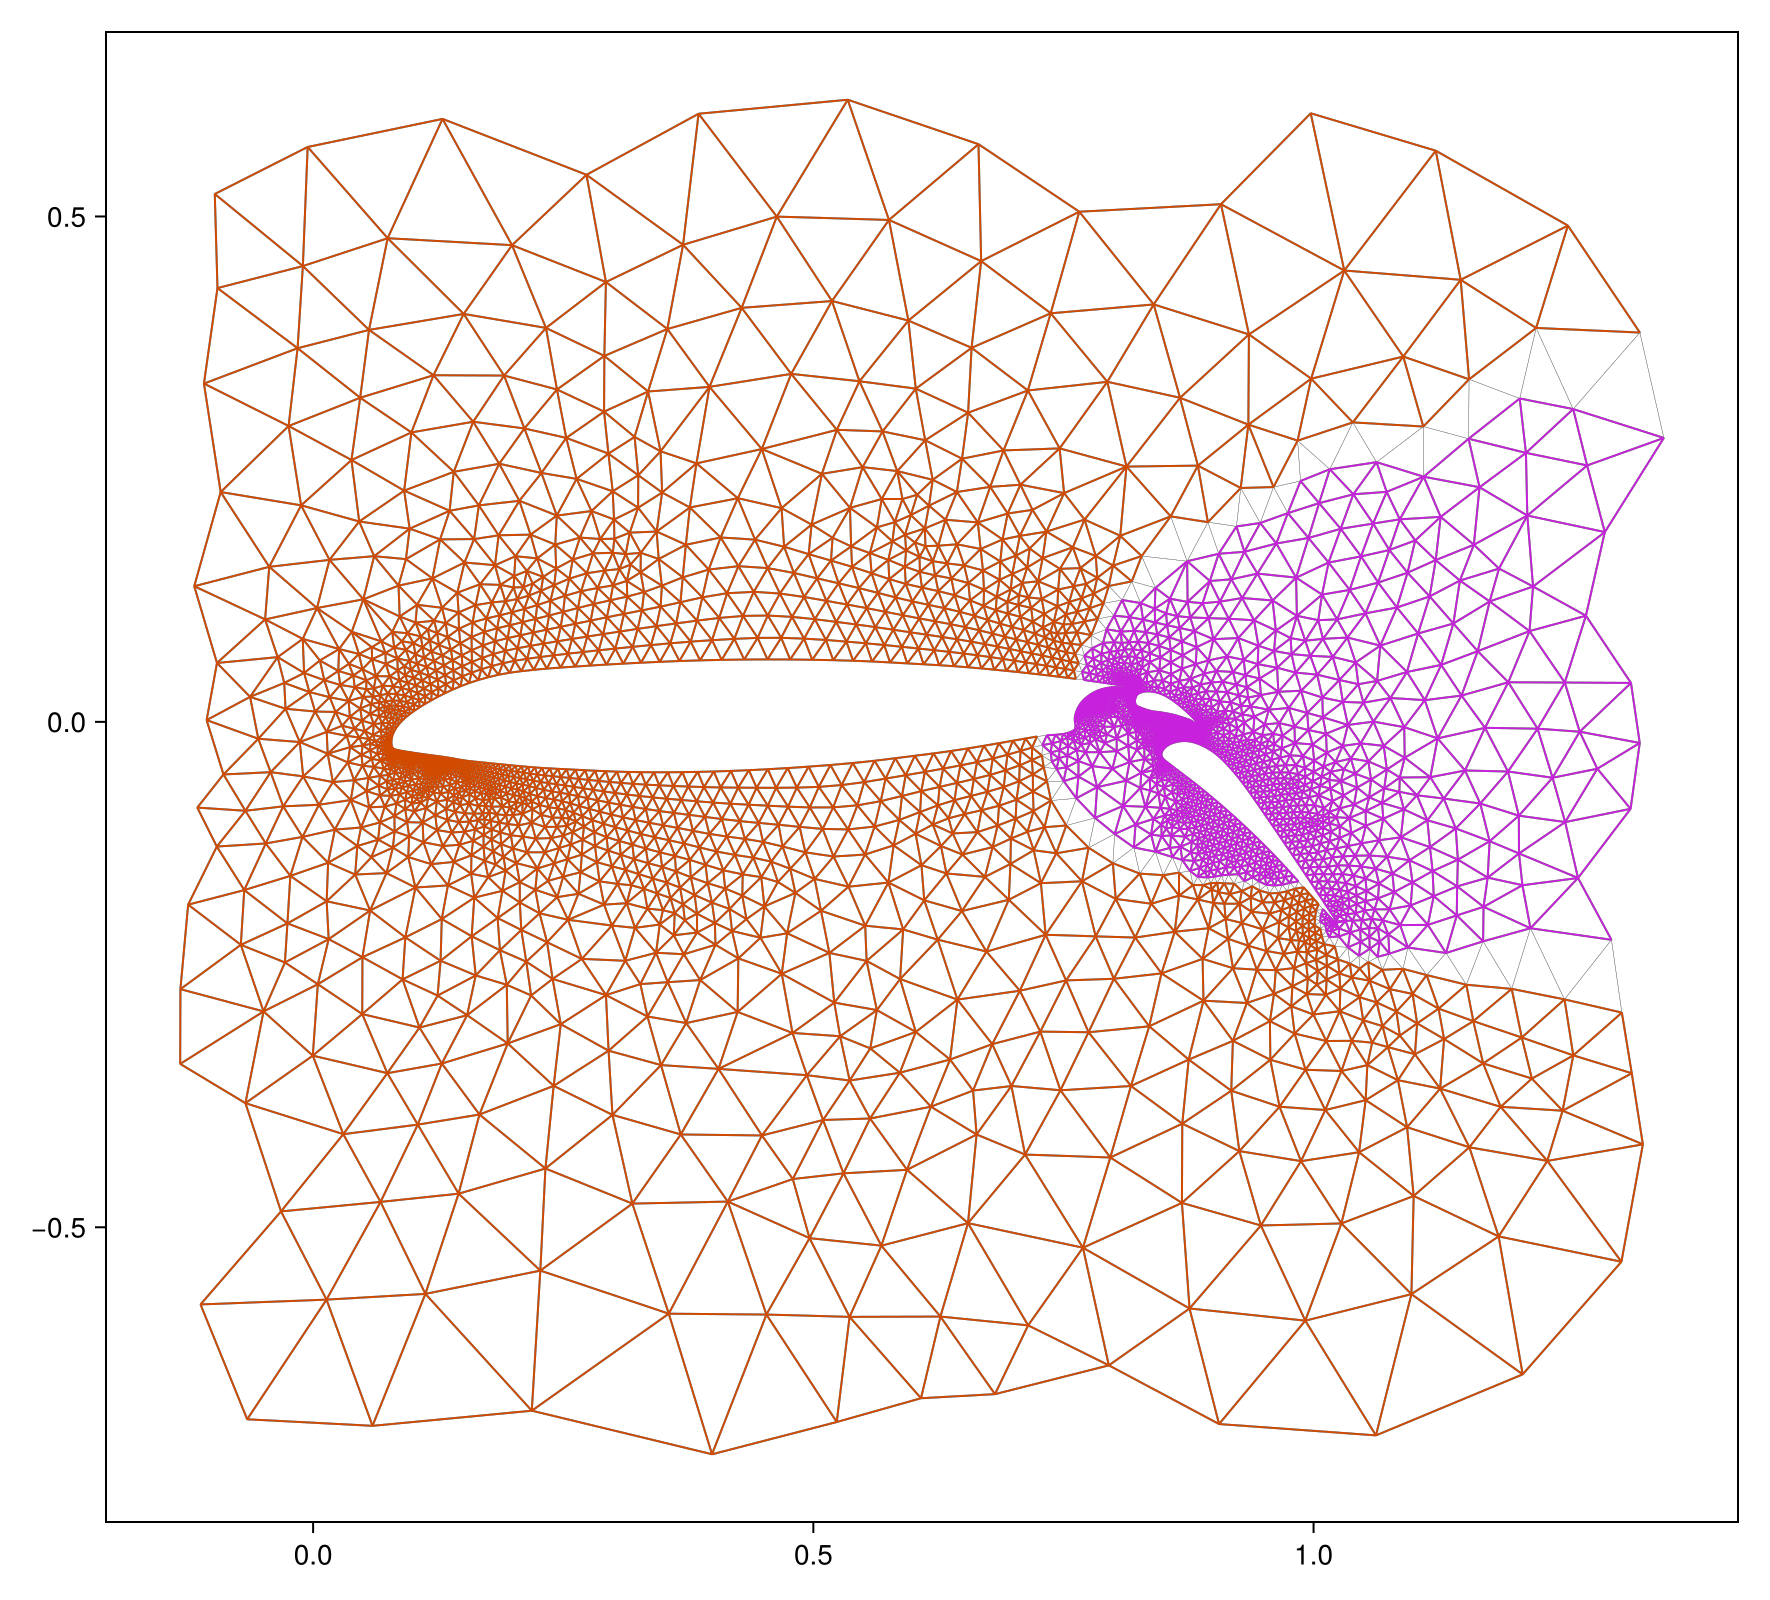
\includegraphics[width=\textwidth,  trim={100pt 74pt 0 0}, clip]{images/ex1_airfoil1_spectral.png}
        \caption{Spectral bisection}
        \label{fig:ex1_spectral}
    \end{subfigure}
    \hfill
    \begin{subfigure}[b]{0.23\textwidth}
        \centering
        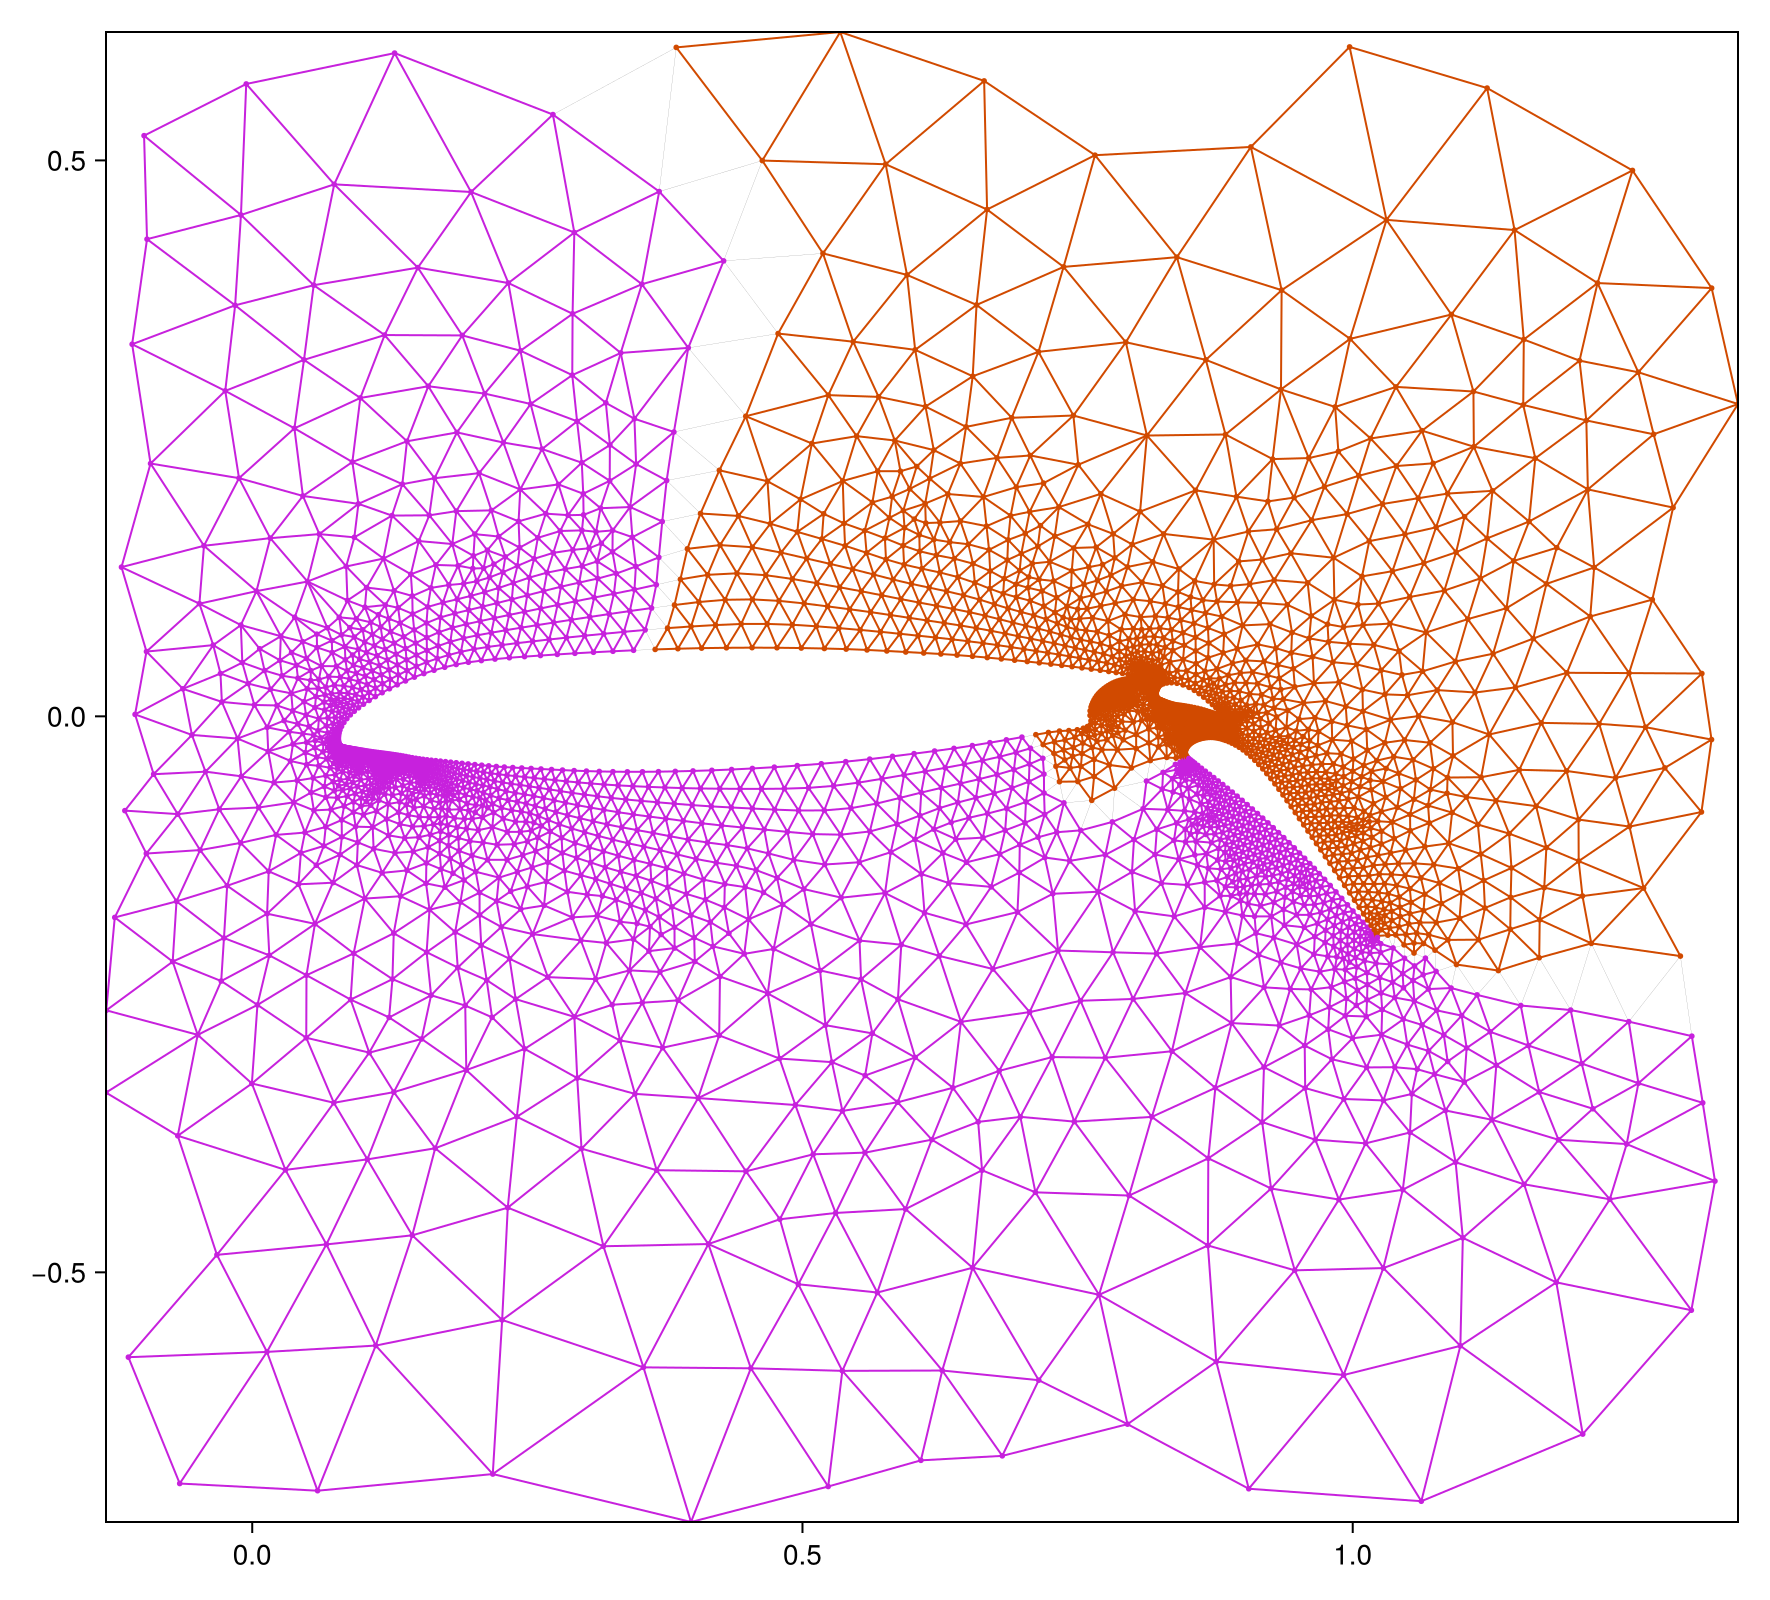
\includegraphics[width=\textwidth,  trim={100pt 74pt 0 0}, clip]{images/ex1_airfoil1_metis.png}
        \caption{Bisection using \texttt{METIS}}
        \label{fig:ex1_metis}
    \end{subfigure}

    \caption{Visualization of four graph bisection methods applied to the \texttt{airfoil1} mesh (4253 nodes and 12289 edges), illustrating differences in partitioning structure and edge cuts.}
    \label{fig:ex1_results}
\end{figure}

%%%%%%%%%%%%%%%%%%%%%%%%%%%%%%%%%%%%%%%%%%%%%%%%%%%%%%%%%%%%%%
% Ex 2
%%%%%%%%%%%%%%%%%%%%%%%%%%%%%%%%%%%%%%%%%%%%%%%%%%%%%%%%%%%%%%
    % \subsubsection{Example 2: Comparing recursive bisection}
    % This example illustrates recursive bisection using multiple methods, including coordinate bisection, inertial bisection, spectral bisection, and recursive bisection via \texttt{METIS} K-way partitioning. The script \texttt{ex2.jl} generates the results presented in \Cref{fig:ex2_results}
    % \begin{figure}[h]
    \centering
    \begin{subfigure}[b]{0.23\textwidth}
        \centering
        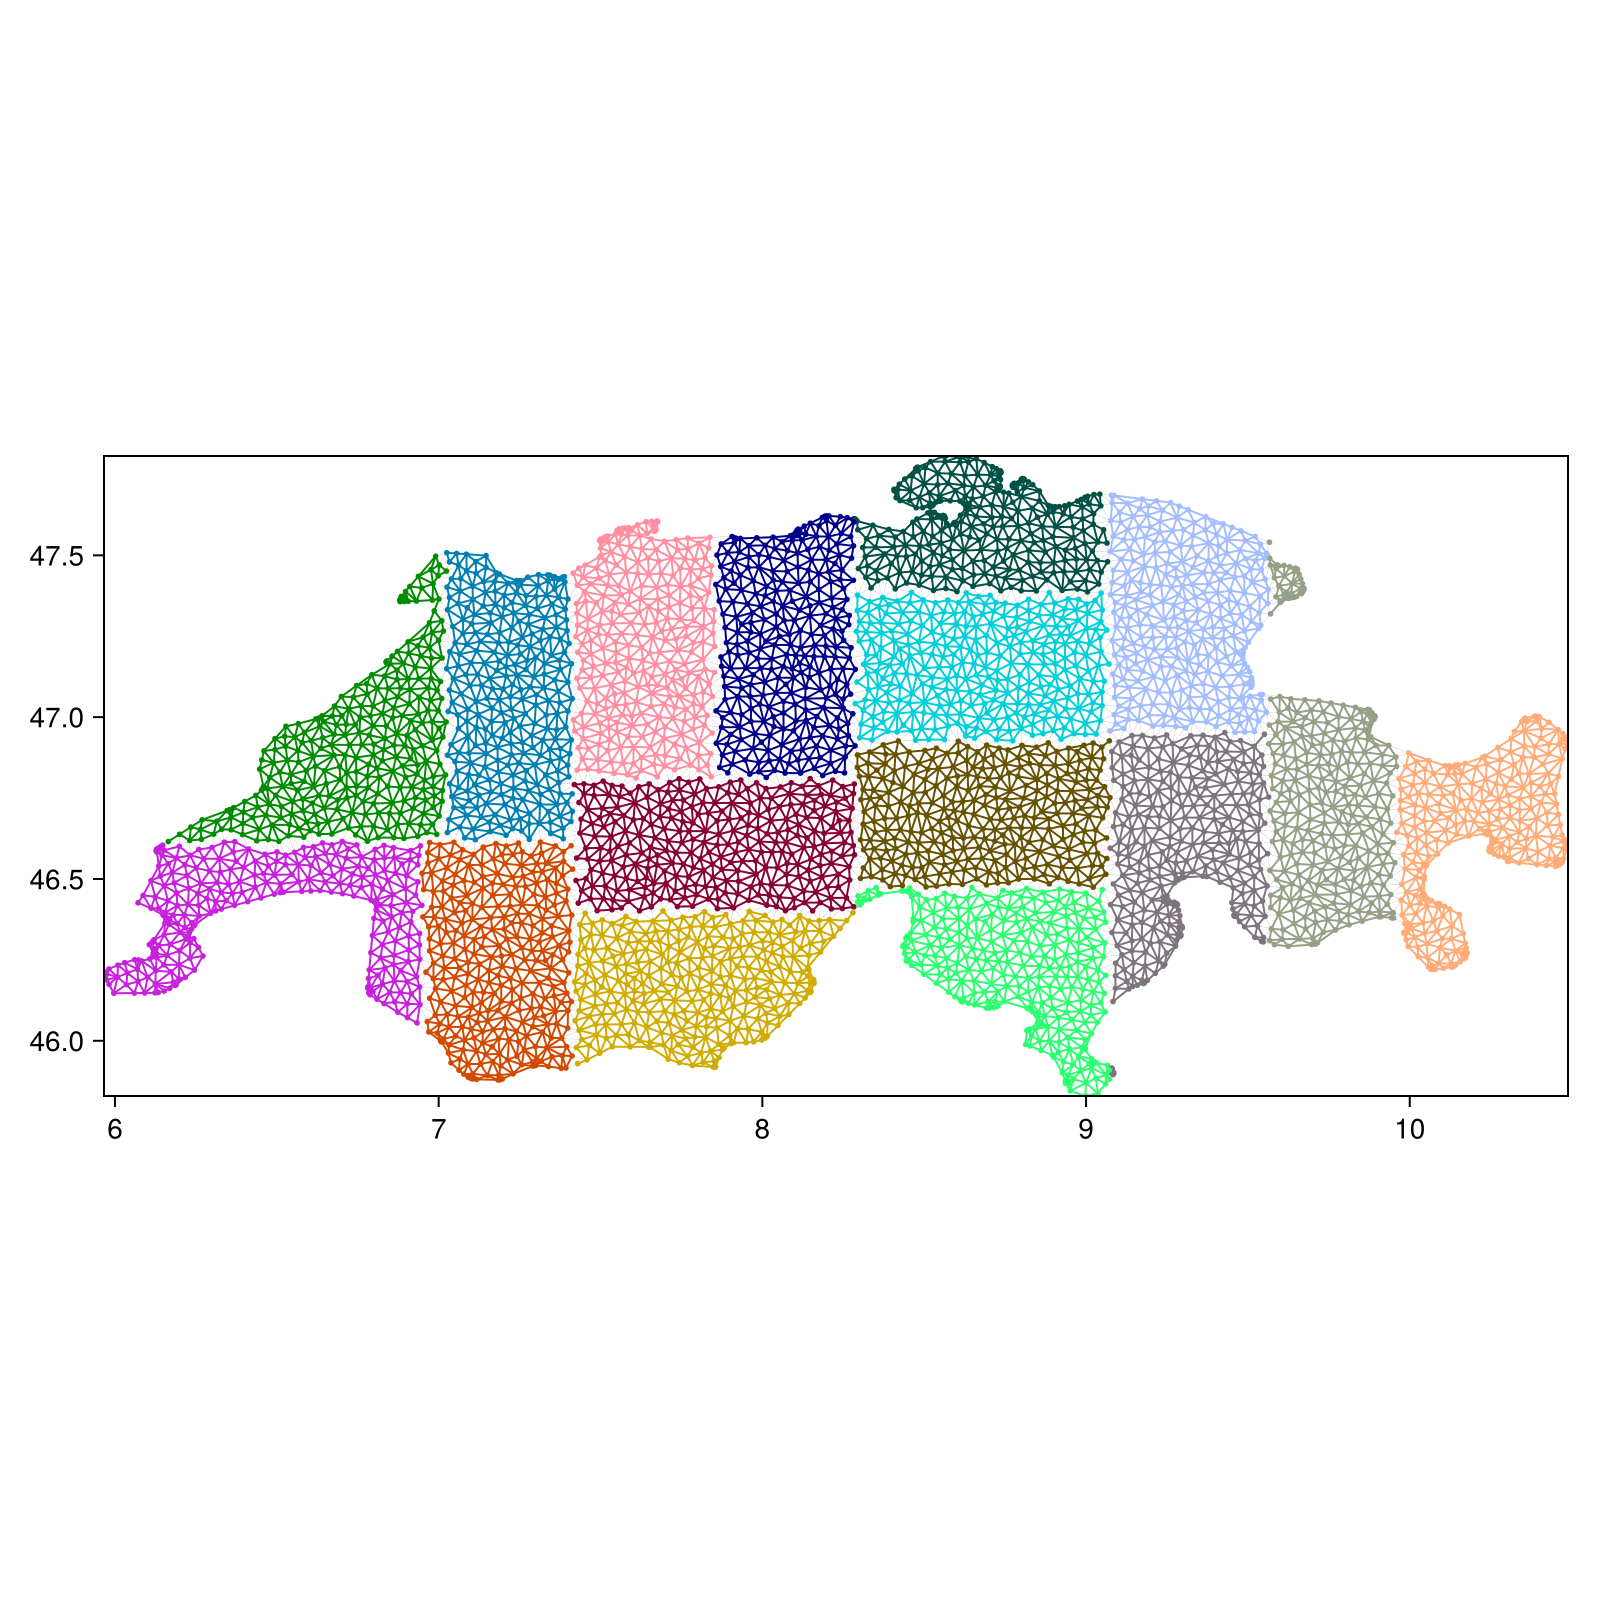
\includegraphics[width=\textwidth,  trim={98pt 70pt 0 0}, clip]{images/ex2_Swiss_graph_coordinate.png}
        \caption{Recursive coordinate bisection}
        \label{fig:ex2_coord}
    \end{subfigure}
    \hfill
    \begin{subfigure}[b]{0.23\textwidth}
        \centering
        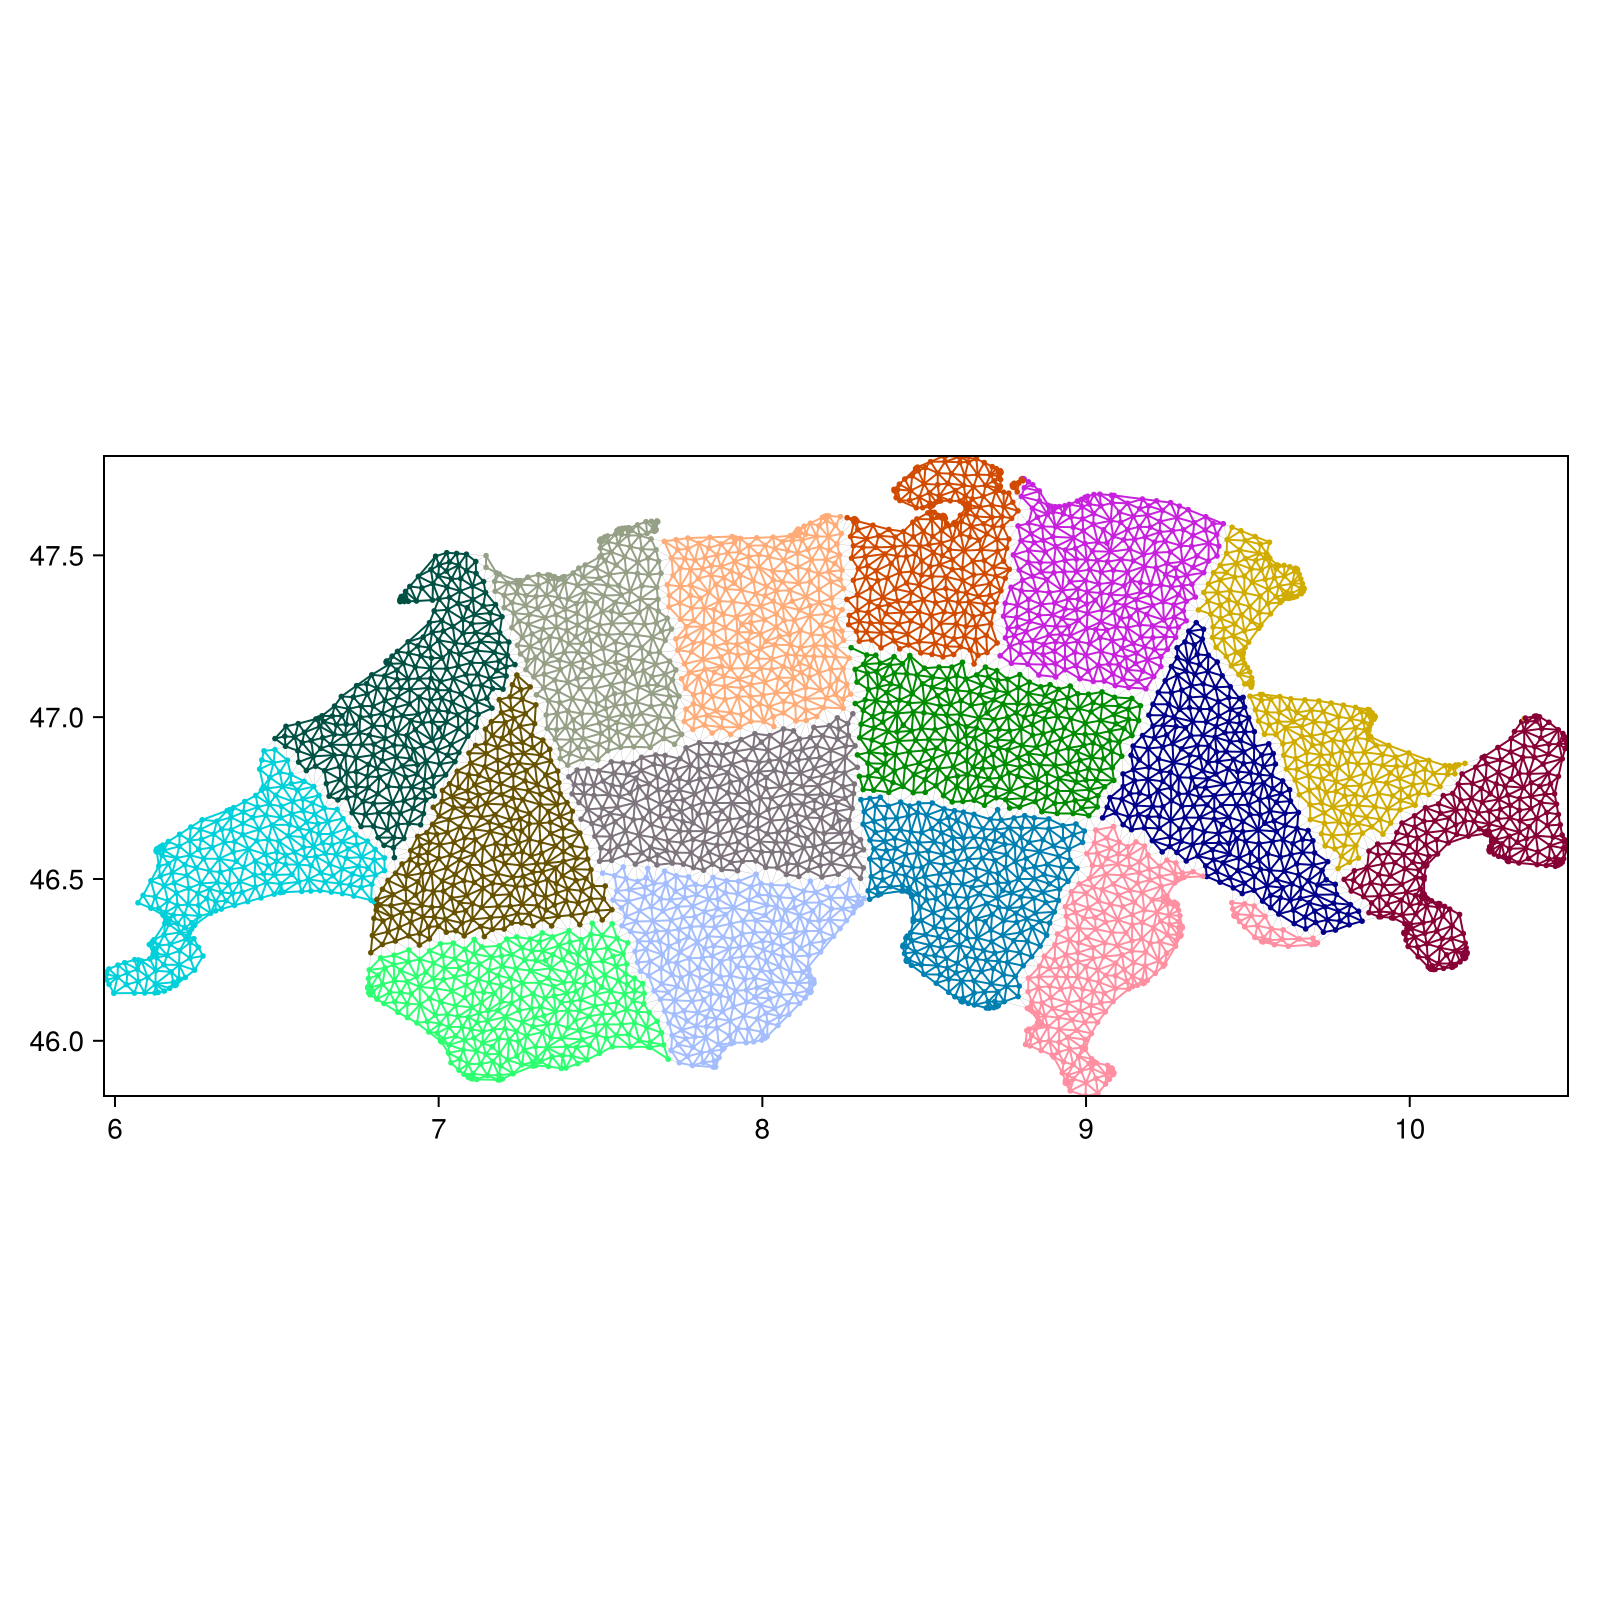
\includegraphics[width=\textwidth,  trim={98pt 70pt 0 0}, clip]{images/ex2_Swiss_graph_inertial.png}
        \caption{Recursive inertial bisection}
        \label{fig:ex2_inertial}
    \end{subfigure}

    \vskip\baselineskip  % Adds vertical space between the rows

    \begin{subfigure}[b]{0.23\textwidth}
        \centering
        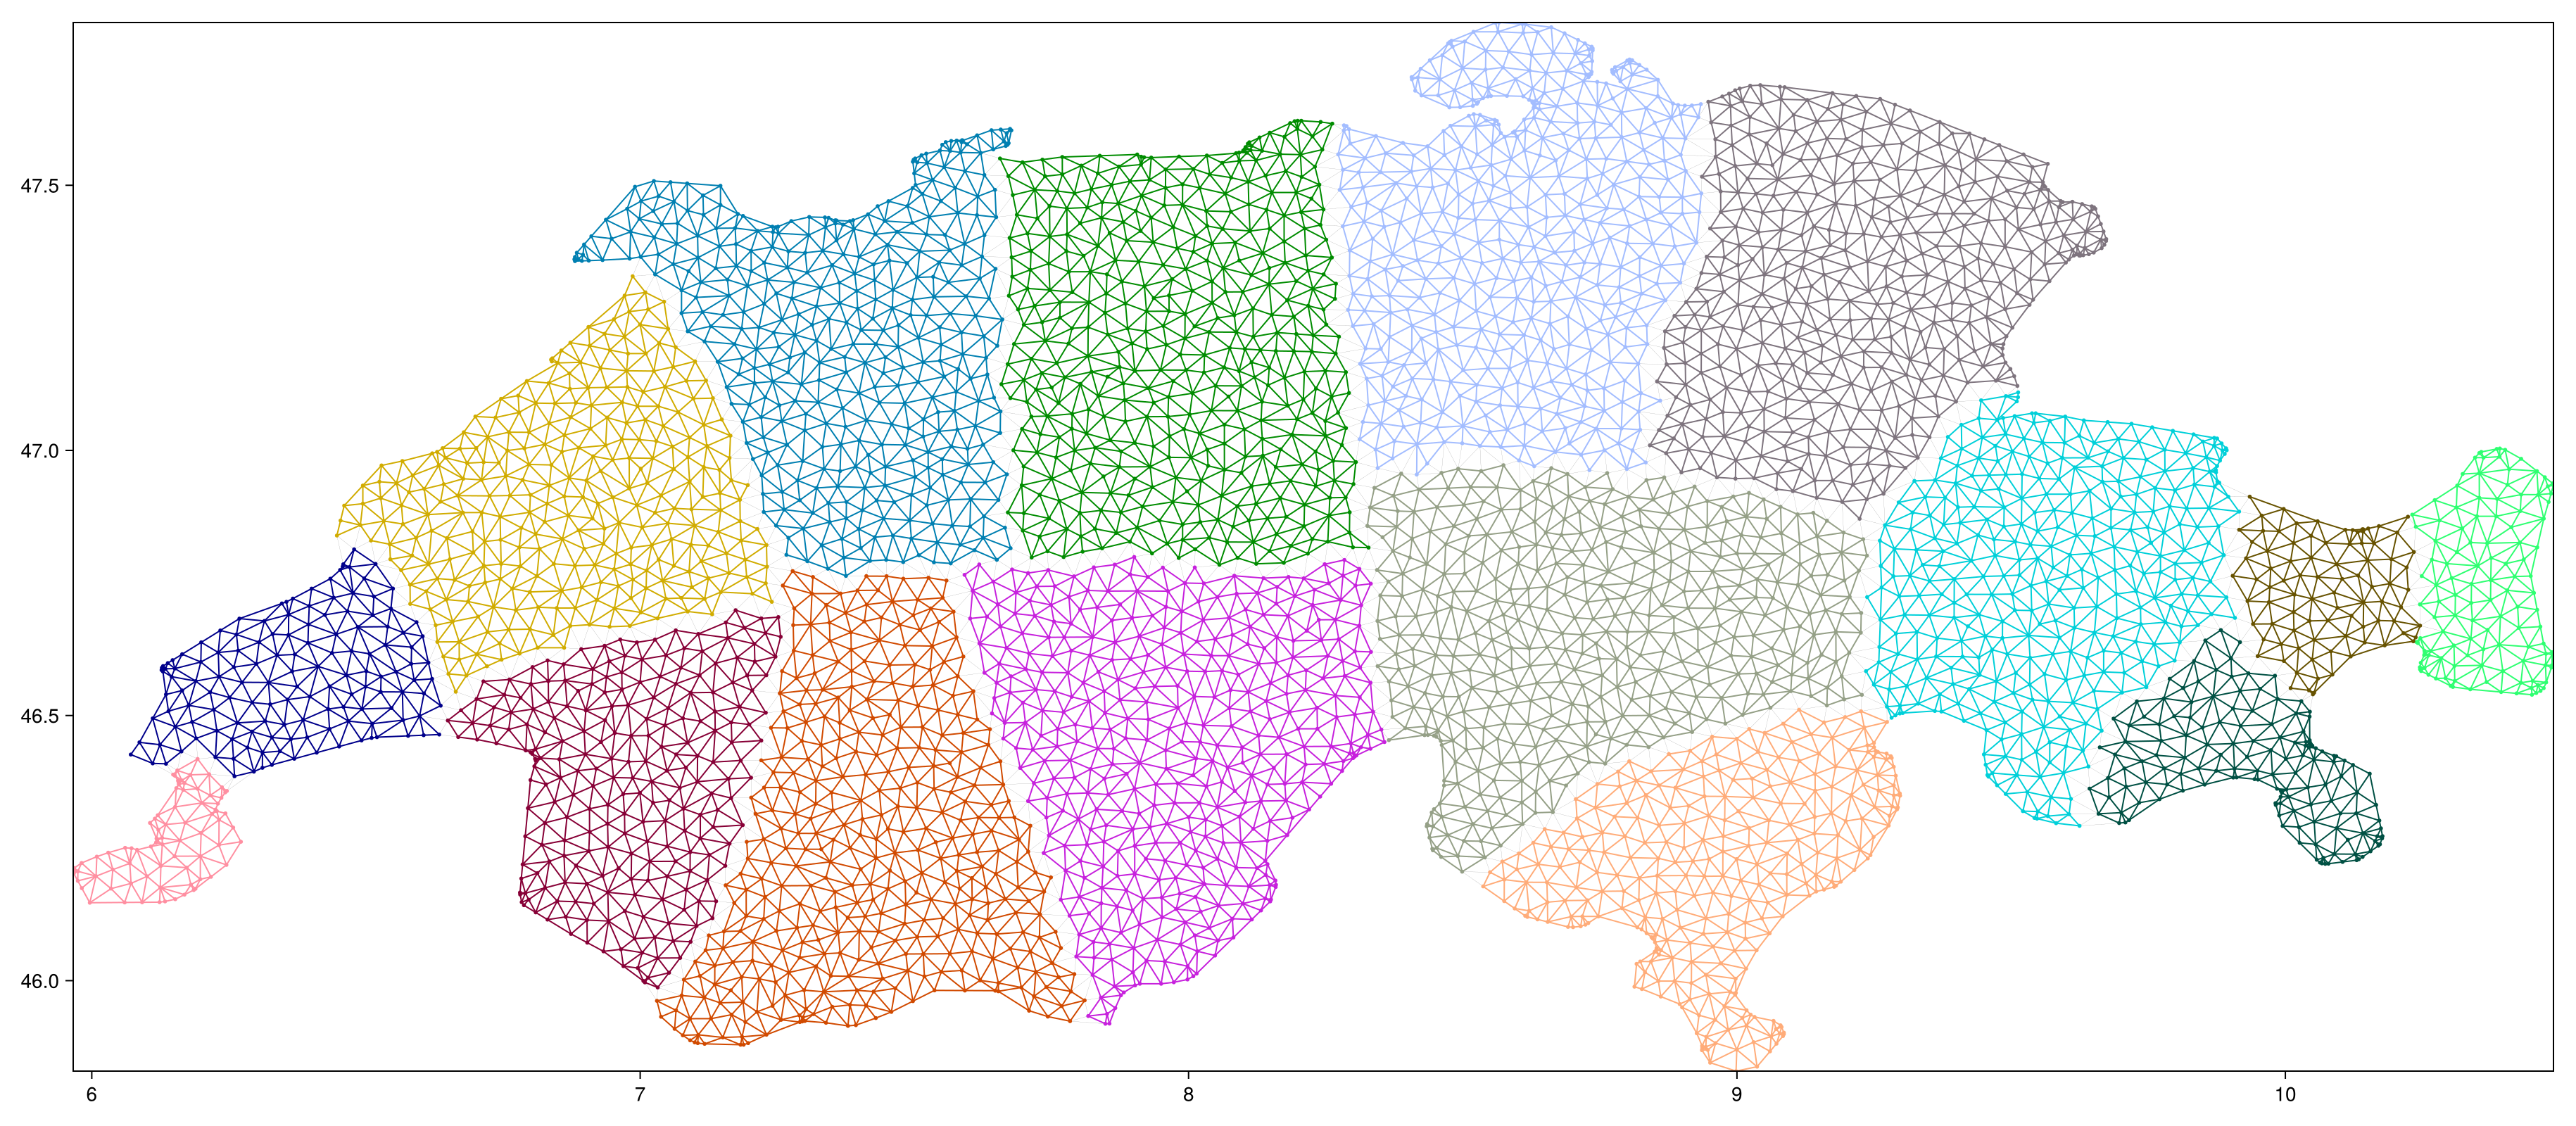
\includegraphics[width=\textwidth,  trim={98pt 70pt 0 0}, clip]{images/ex2_Swiss_graph_spectral.png}
        \caption{Recursive spectral bisection}
        \label{fig:ex2_spectral}
    \end{subfigure}
    \hfill
    \begin{subfigure}[b]{0.23\textwidth}
        \centering
        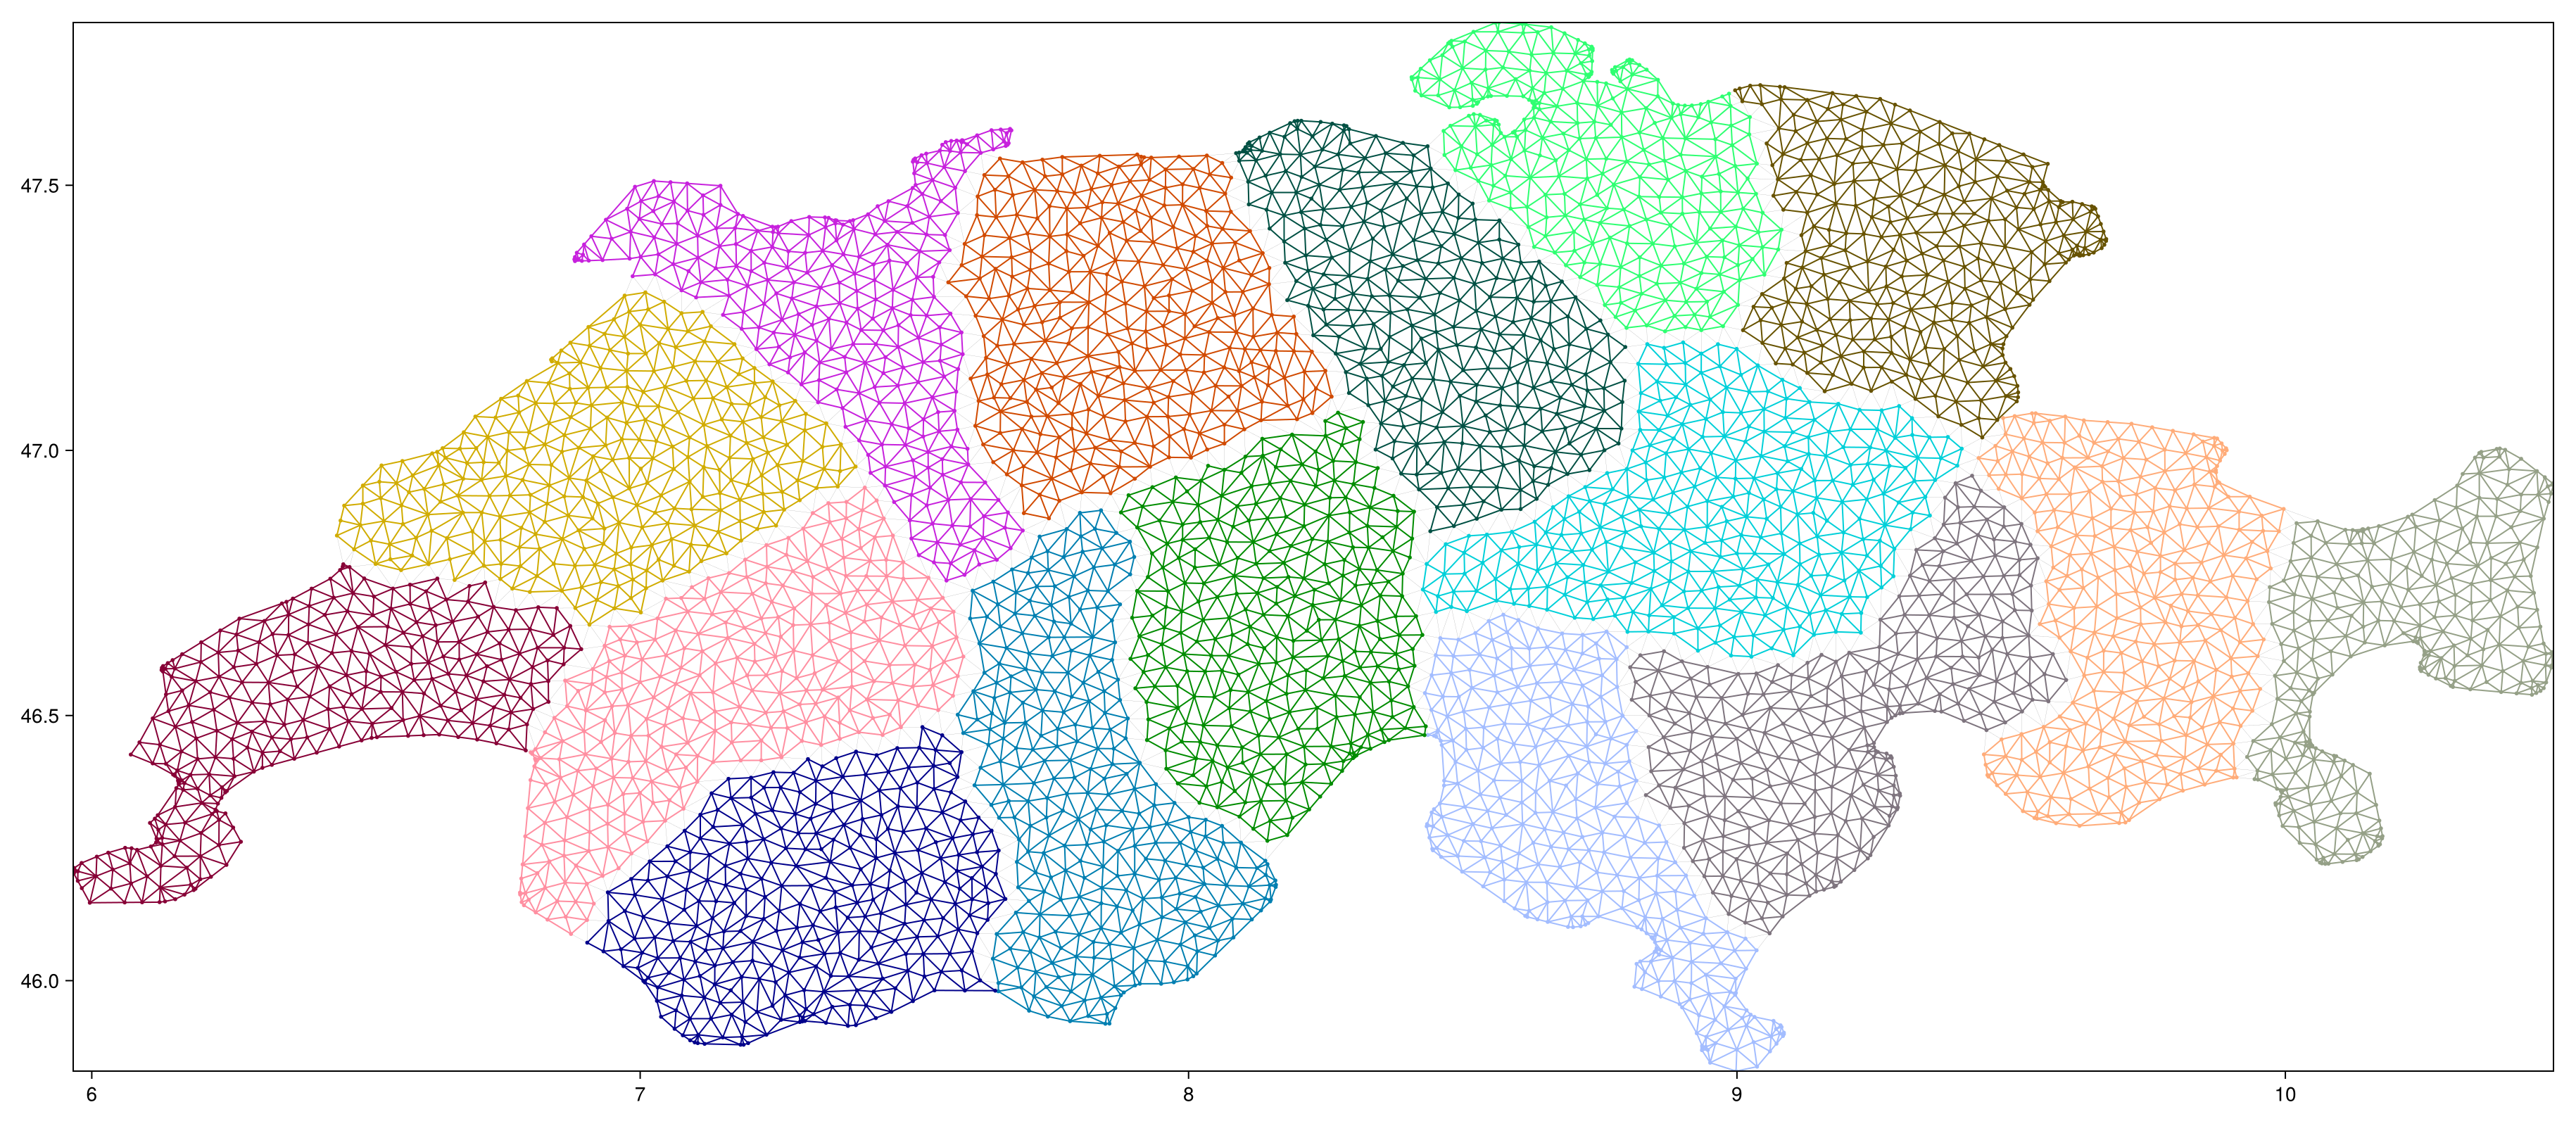
\includegraphics[width=\textwidth,  trim={98pt 70pt 0 0}, clip]{images/ex2_Swiss_graph_metis_rec.png}
        \caption{Recursive \texttt{METIS} bisection}
        \label{fig:ex2_metis}
    \end{subfigure}

    \caption{Comparison of four graph recursive bisection methods applied to the \texttt{Swiss\_graph} (4468 nodes and 15230 edges), illustrating differences in recursive partitioning results.}
    \label{fig:ex2_results}
\end{figure}


% \begin{figure}
%     \centering

%     \begin{subfigure}[b]{0.45\textwidth}
%         \centering
%         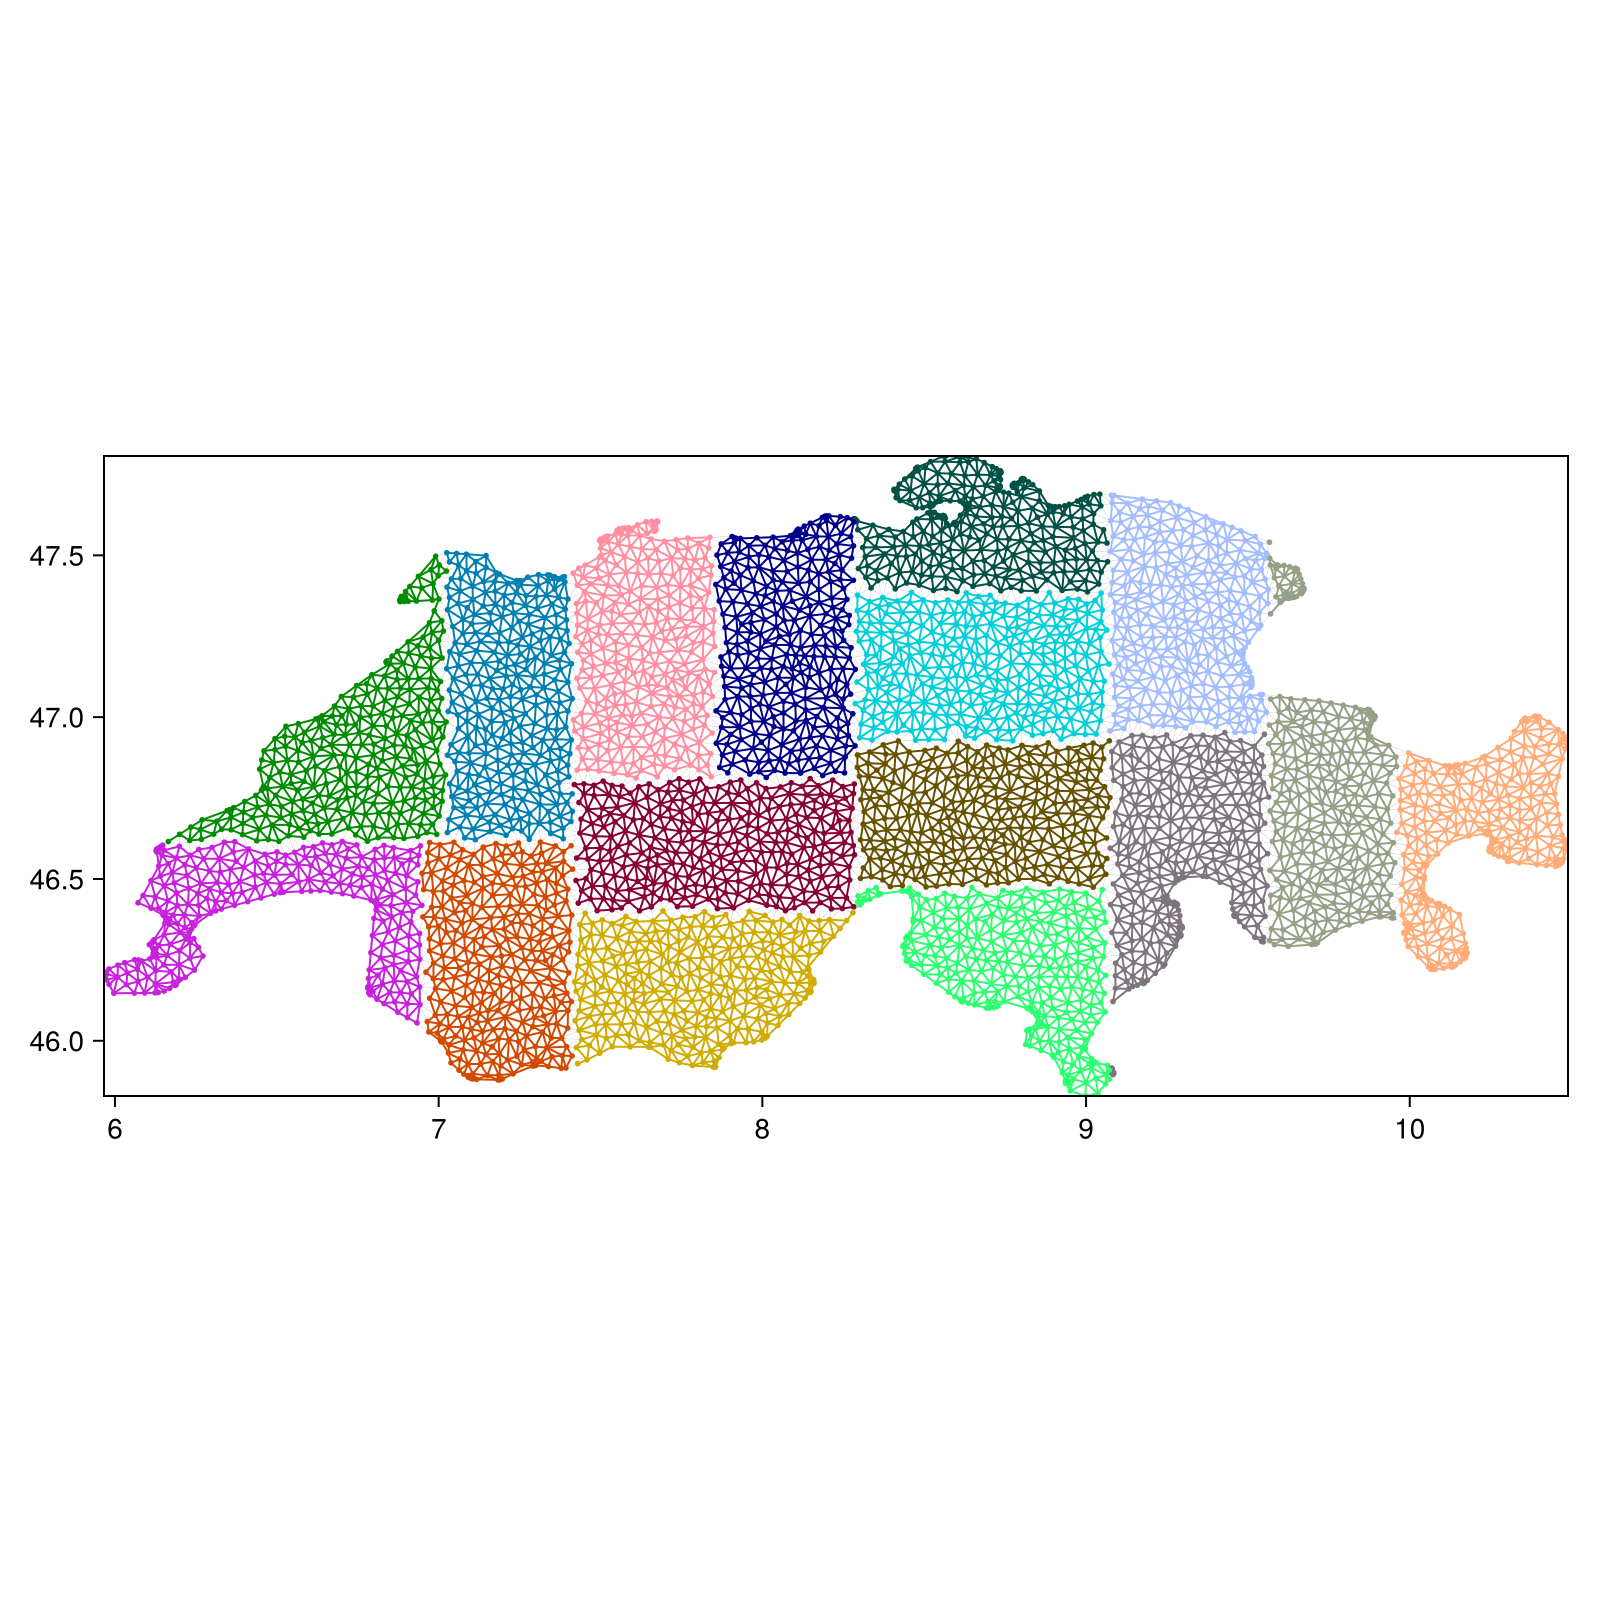
\includegraphics[width=\textwidth, trim={98pt 70pt 0 0}, clip]{images/ex2_Swiss_graph_coordinate.png}
%         \caption{Recursive coordinate bisection}
%         \label{fig:ex2_coord}
%     \end{subfigure}

%     \vskip\baselineskip

%     \begin{subfigure}[b]{0.45\textwidth}
%         \centering
%         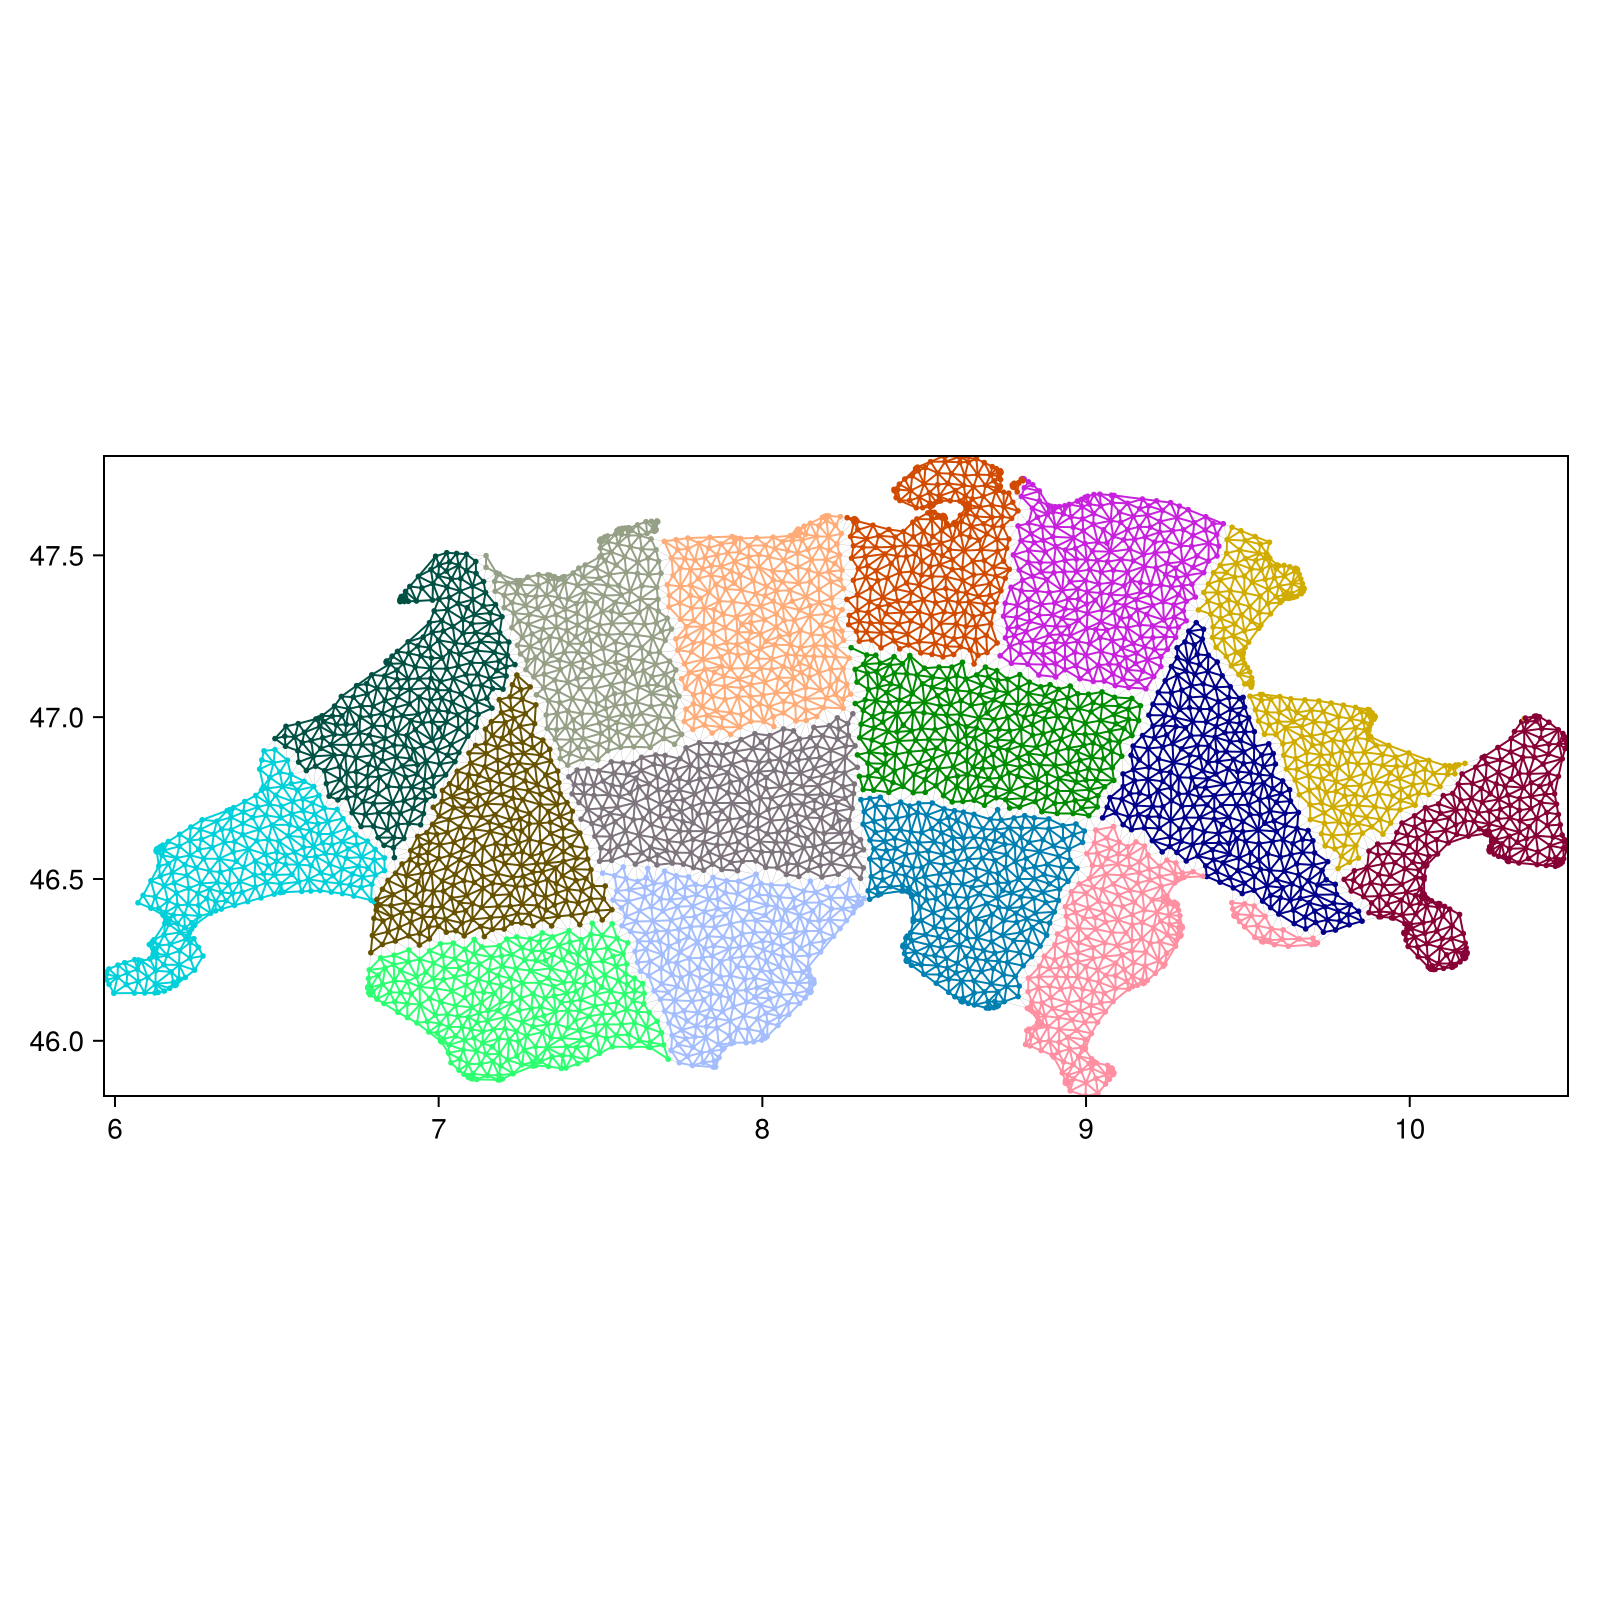
\includegraphics[width=\textwidth, trim={98pt 70pt 0 0}, clip]{images/ex2_Swiss_graph_inertial.png}
%         \caption{Recursive inertial bisection}
%         \label{fig:ex2_inertial}
%     \end{subfigure}

%     \vskip\baselineskip

%     \begin{subfigure}[b]{0.45\textwidth}
%         \centering
%         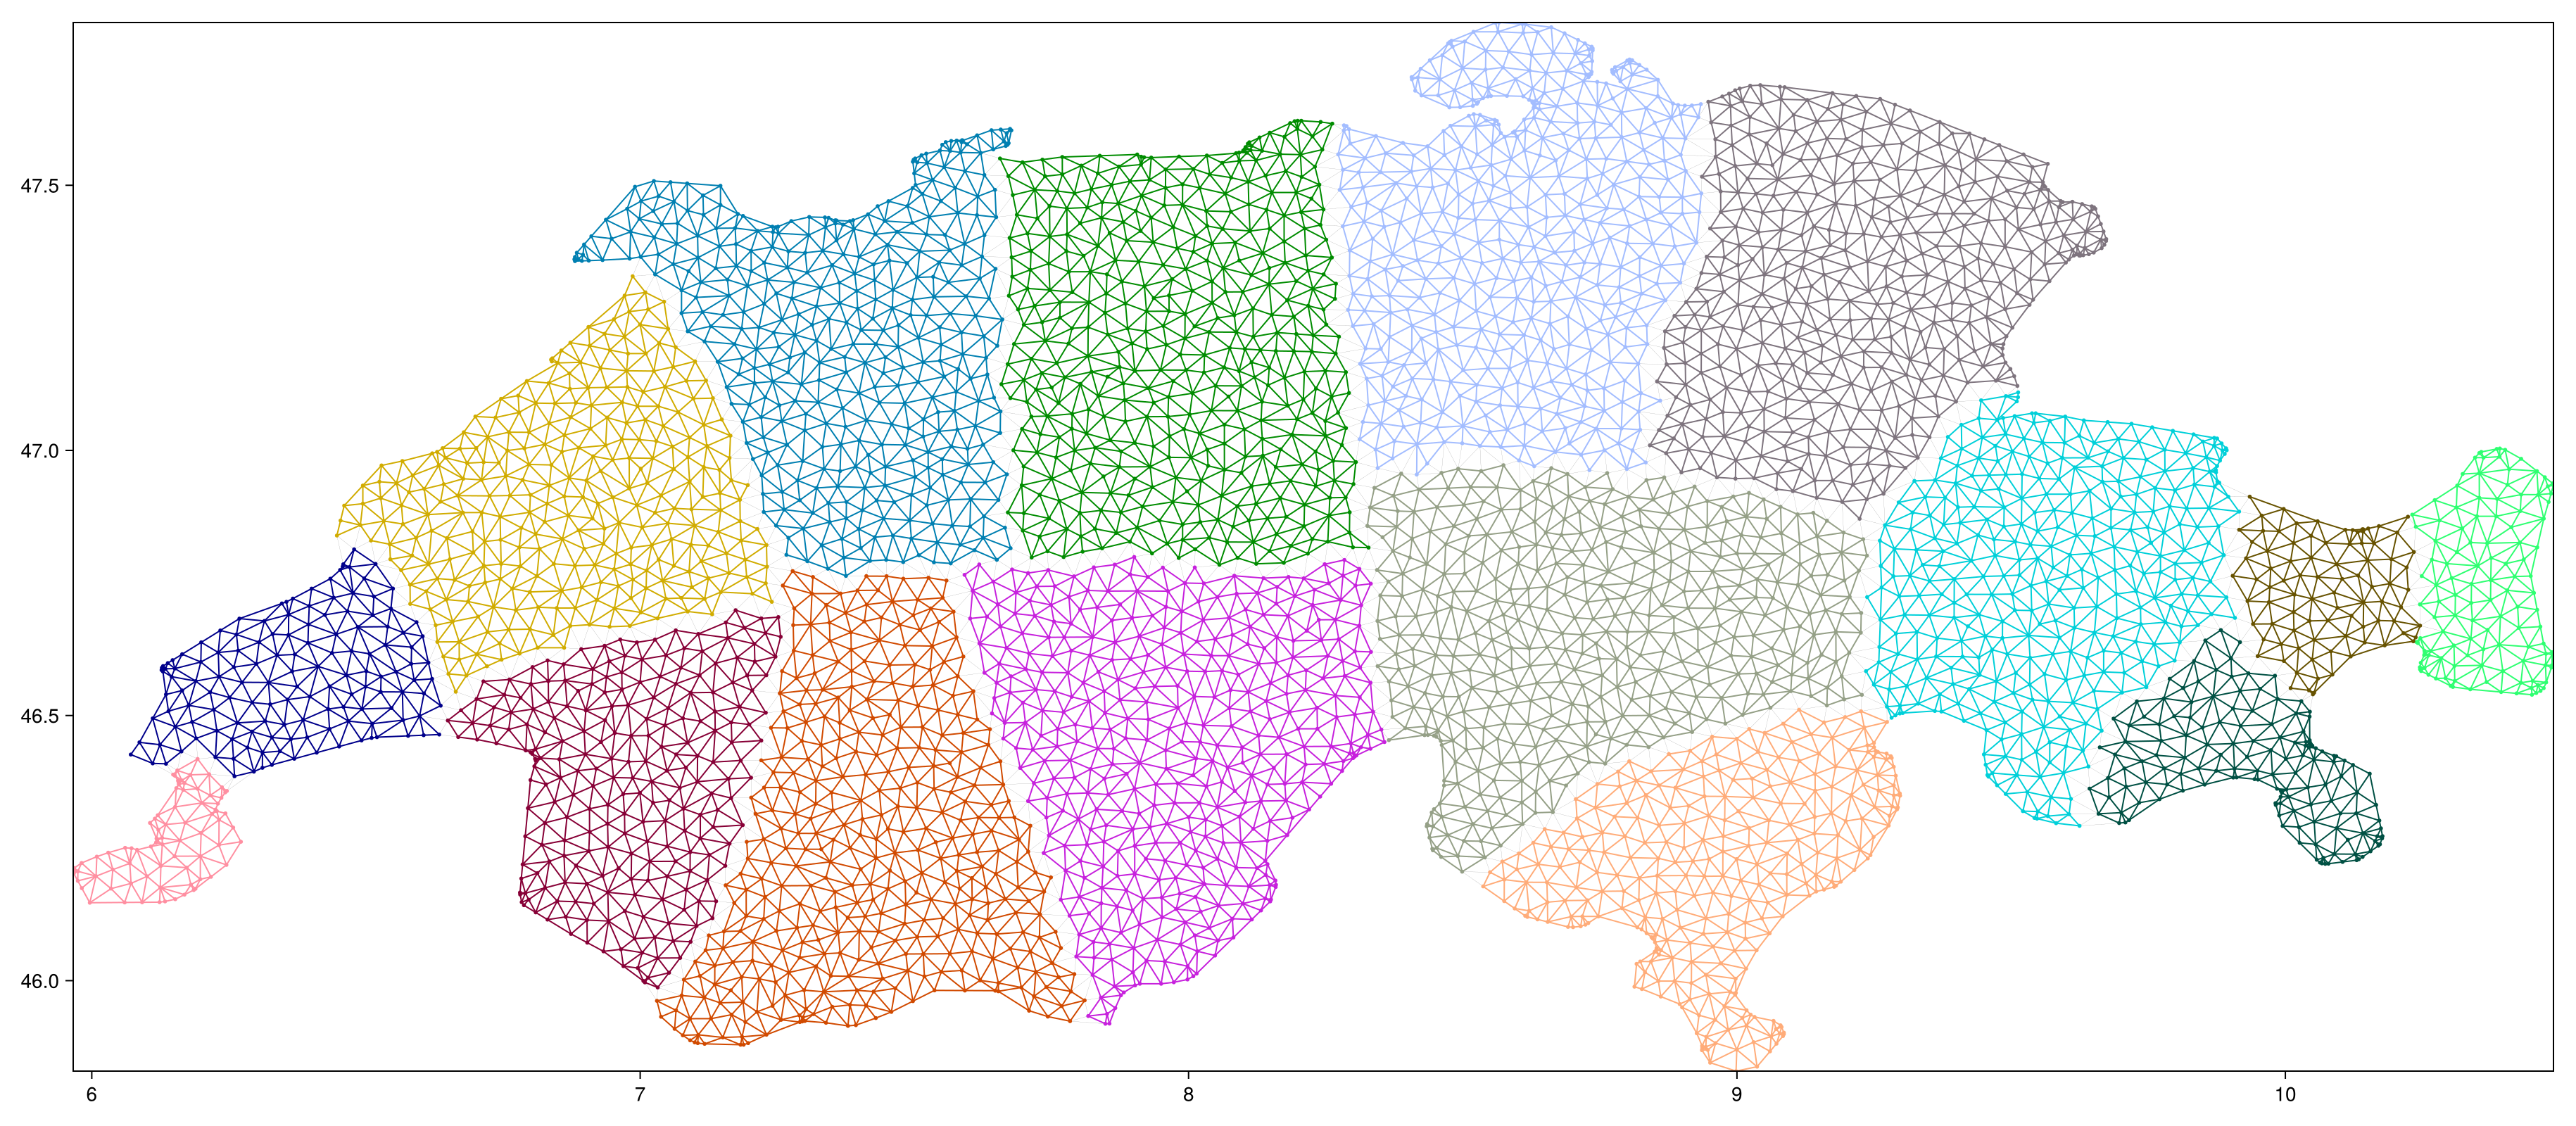
\includegraphics[width=\textwidth, trim={98pt 70pt 0 0}, clip]{images/ex2_Swiss_graph_spectral.png}
%         \caption{Recursive spectral bisection}
%         \label{fig:ex2_spectral}
%     \end{subfigure}

%     \vskip\baselineskip

%     \begin{subfigure}[b]{0.45\textwidth}
%         \centering
%         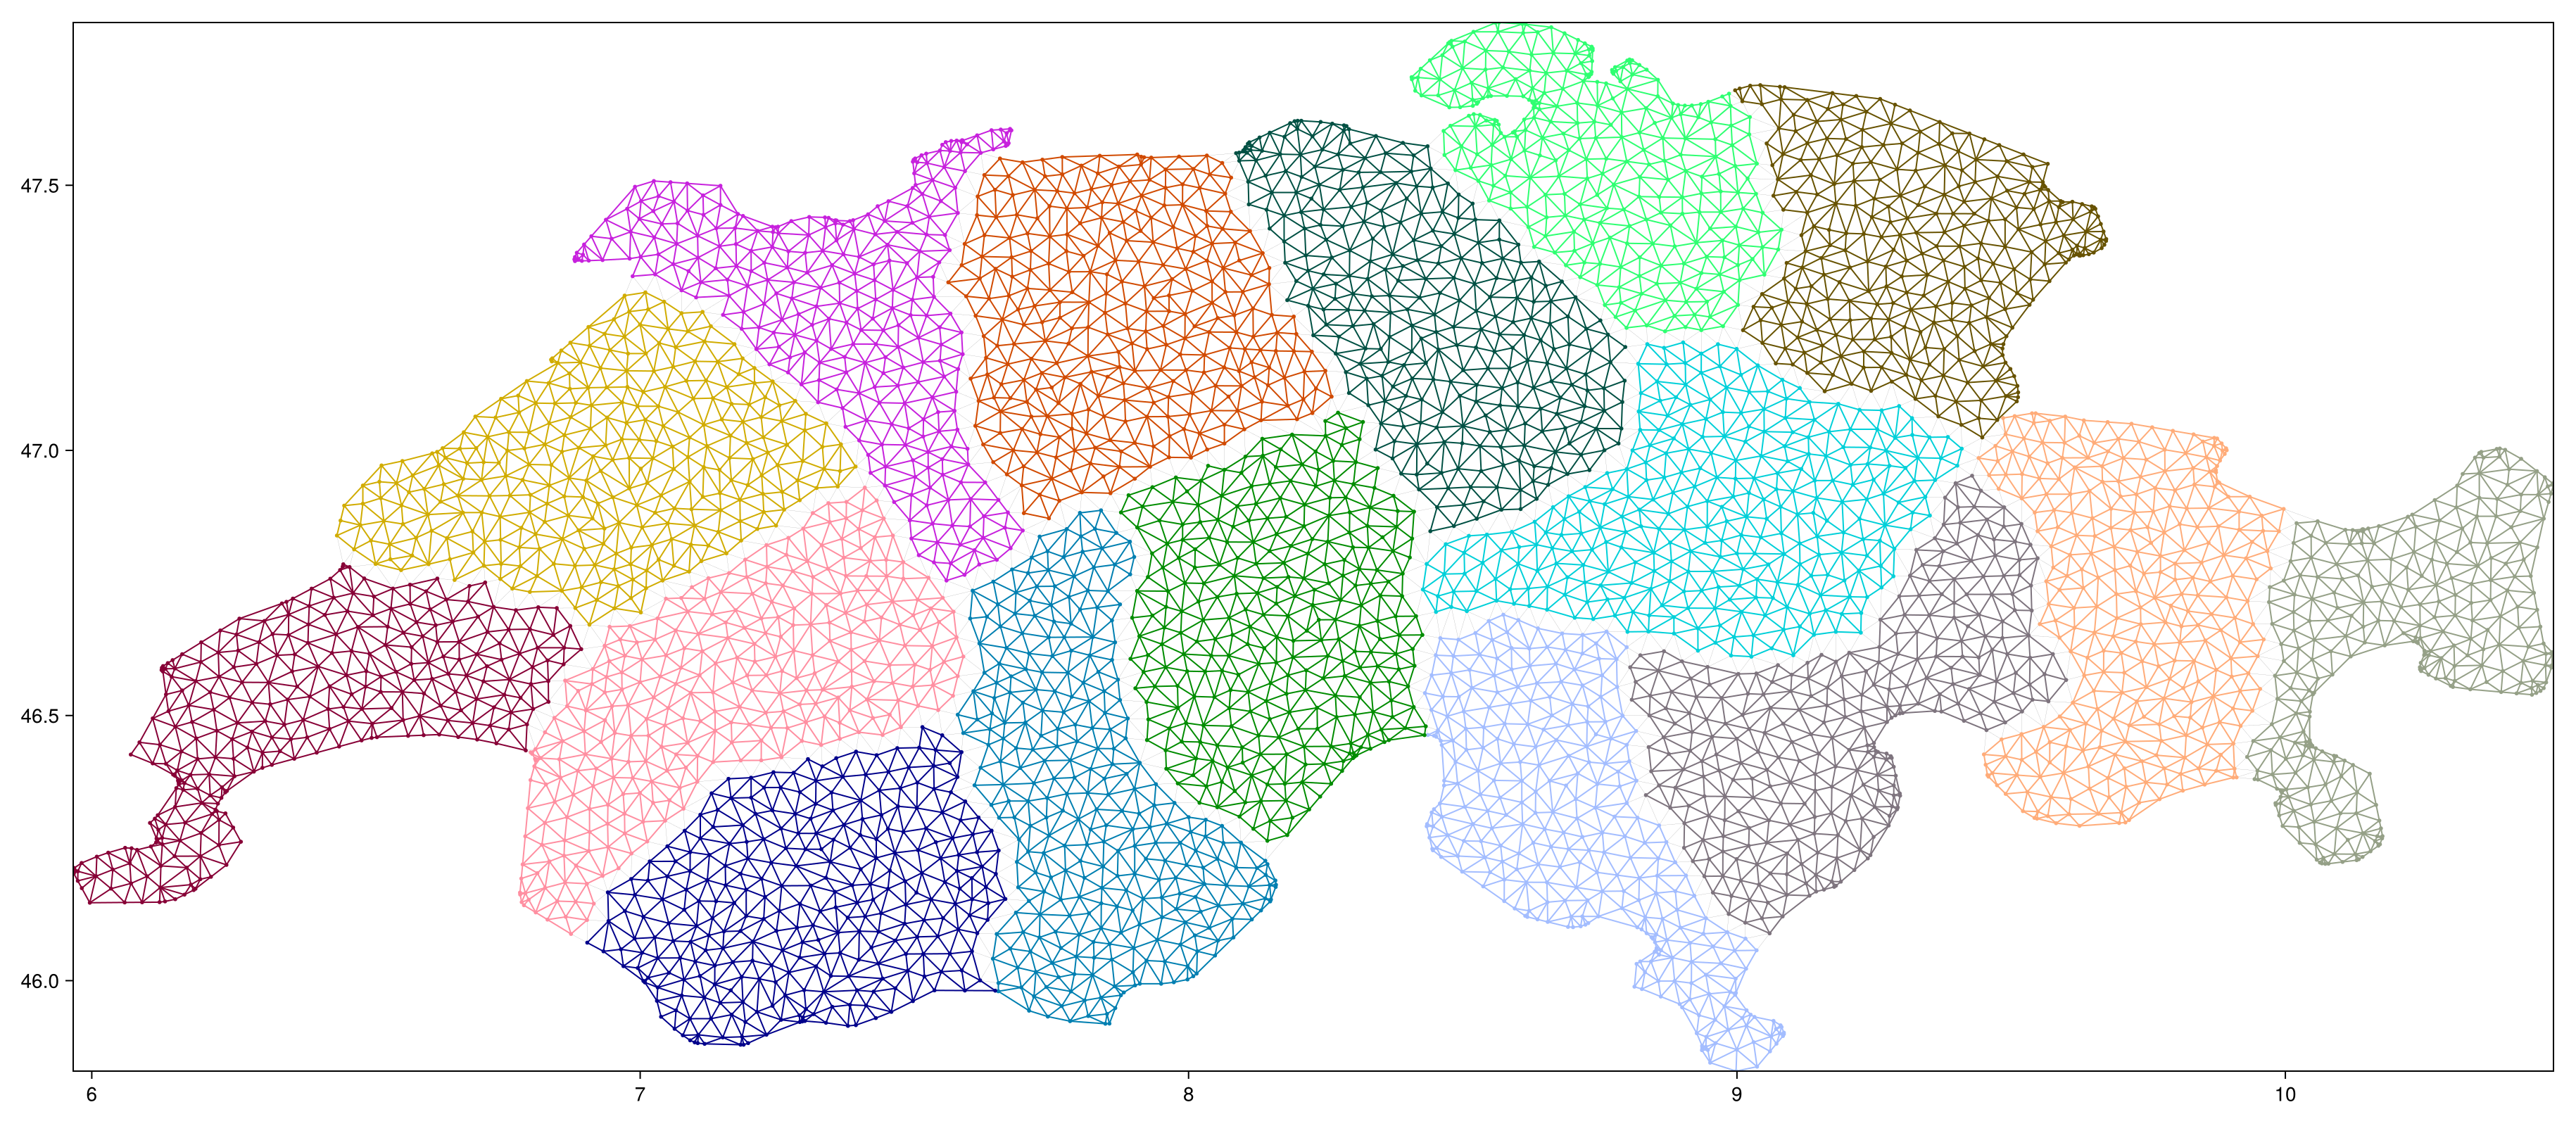
\includegraphics[width=\textwidth, trim={98pt 70pt 0 0}, clip]{images/ex2_Swiss_graph_metis_rec.png}
%         \caption{Recursive spectral bisection}
%         \label{fig:ex2_metis}
%     \end{subfigure}

%     \caption{Recursive bisection of the \texttt{Swiss\_graph} mesh using different methods. Each partition result shows the division into $p = 16$ subdomains.}
%     \label{fig:ex2_results}
% \end{figure}

%%%%%%%%%%%%%%%%%%%%%%%%%%%%%%%%%%%%%%%%%%%%%%%%%%%%%%%%%%%%%%
% Usage in teaching scenarios
%%%%%%%%%%%%%%%%%%%%%%%%%%%%%%%%%%%%%%%%%%%%%%%%%%%%%%%%%%%%%%
    % \subsection{Usage in teaching scenarios}
    % \texttt{GraphLab.jl} is designed to support educational use, particularly in courses covering graph algorithms, high-performance computing, and scientific computing.
    % By offering an interactive and reproducible environment, the package enables students to experiment with various partitioning techniques, assess their performance, and gain intuition about graph bisection methods.

    % A typical teaching application could involve \texttt{Pluto.jl} or Google Colab notebooks for visualizing and comparing partitioning methods.
    % For instance, an instructor can guide students through partitioning sample meshes, examining the effects of different algorithms on edge cut and balance ratio.
\end{document}

